\documentclass[11pt]{article}

\usepackage{amsmath}
\usepackage{amssymb}
\usepackage{geometry}
\usepackage[hidelinks,hypertexnames=false]{hyperref}
\usepackage{booktabs}
\usepackage{array}
\usepackage{longtable}
\usepackage{float}
\usepackage{placeins}
\usepackage{pgfplots}

\pgfplotsset{compat=1.18}
\newcolumntype{P}[1]{>{\raggedright\arraybackslash}p{#1}}
\hbadness=10000
\vbadness=10000
\hfuzz=2pt
% Permit limited additional line-breaking flexibility instead of accepting
% paragraphs that intrude into the 1-inch body-text margins.
\emergencystretch=2em
\vfuzz=30pt

\geometry{margin=1in}

\newcommand{\clip}{\operatorname{clip}}

\title{A Dynamic, Decomposable Operational Cyber Risk Posture Index}
\author{James Booth}
\date{28 October 2026 \\ Pre-submission Review Draft v0.2}

\begin{document}
\maketitle

\begin{abstract}
  Cybersecurity risk is inherently dynamic, multi-dimensional, and shaped by the
  continuous interaction between technology, adversary capability, organizational
  behavior, and dependency structure. While architectures, tooling, and governance
  frameworks evolve rapidly, the executive questions remain stable: \emph{What is our
  current risk posture? What is driving it? How exposed are we, how severe would impact
  be, and how quickly can we detect, respond, and recover?}

  This paper introduces the Cyber Risk Posture Index (CRPI), a telemetry-compatible,
  framework-agnostic, decomposable operational posture index for representing
  organizational cyber risk as a function of time. The governing model is
  mathematically specified rather than based on discretionary top-level scoring: threat
  exposure is combined with resilience-adjusted consequence, operational execution is
  modulated by observability, and past unresolved exposure is represented by a
  bounded stock-flow state. In this representation, current residual exposure
  contributes to a persistent score over time, effective mitigation reduces that
  score, and the state remains between zero and one. It is a modeled measure of
  unresolved exposure, not a directly observed vulnerability count. Regularized geometric aggregation prevents a
  single zero-valued sub-metric from unintentionally collapsing an otherwise non-zero
  construct. The model produces a bounded, scope-aware operational risk metric together with
  traceable diagnostics for hazard pressure, mitigation effectiveness, instantaneous
  residual posture, and persistent unresolved exposure. Subjectivity is not claimed to
  be eliminated; it is constrained to explicit, versioned composition and calibration
  parameters. The paper further specifies measurement interfaces, evidence-coverage
  gates, uncertainty propagation, calibration governance, and implementation-oriented
  sub-metrics as a reproducible foundation for subsequent empirical validation.
\end{abstract}

\section{Introduction}
\label{sec:intro}
At the executive and board level, cybersecurity is ultimately a risk management
problem. Senior leaders repeatedly ask a small number of fundamental questions:
\emph{How risky are we today? What is our current exposure? What is the likelihood of
meaningful impact? If something happens, how effectively can we detect it, contain it,
and recover?} Despite substantial investment in security programs and tooling, these
questions are rarely answered with quantitative clarity that is both trustworthy and
traceable.

Most existing approaches to cyber risk assessment rely on static, point-in-time
evaluations, qualitative scoring, control-centric dashboards, or framework-specific
maturity models. While such approaches are valuable for compliance, assurance, and
control management, they struggle to represent risk as a continuously evolving
property of a living socio-technical system. As new technologies emerge and
adversaries adapt, models that encode technology-specific assumptions can lose
explanatory power or become difficult to compare across time, business units, and
organizations \cite{nist-csf,nist80030,iso27001,iso27005,cis-controls,fair-book,cvss31,cvss40}.

This work proposes a different approach: a small set of stable, mathematically
specified equations operating over cyber-risk constructs whose semantics remain useful
across different technologies and governance frameworks. The Cyber Risk Posture Index (CRPI)
is not intended to estimate breach probability or monetary loss. It is an operational
posture index designed to convert heterogeneous evidence into a bounded, decomposable,
time-aware representation of current and persistent residual exposure. Mathematical
grounding reduces reliance on discretionary top-level weights, while explicit
calibration governance makes the remaining judgment visible, local, versioned, and
auditable.

The paper makes five specific contributions:
\begin{enumerate}
  \item it defines a technology-agnostic set of Tier~2 cyber-risk constructs separating
    observability, consequence, threat exposure, operational execution, and resilience;
  \item it specifies a zero-safe regularized aggregation operator that preserves
    geometric sensitivity to weak components without allowing one zero-valued input to
    collapse an otherwise non-zero construct;
  \item it introduces explicit equations for resilience-adjusted consequence,
    observability-modulated mitigation, instantaneous residual posture, and bounded
    stock-flow persistence rather than relying on discretionary top-level weights;
  \item it provides measurement, coverage, uncertainty, and governance interfaces for
    mapping heterogeneous telemetry into stable normalized constructs; and
  \item it demonstrates how AI-era changes in public threat signals can be represented
    without treating temporal correlation as proof that AI produced the observed
    change.
\end{enumerate}

\subsection*{Organization of the research}
The paper first establishes the operational concepts and five measurable dimensions of
posture, then explains how their evidence is qualified and how changing conditions can
carry effects across reporting periods. With that vocabulary established, it introduces
the governing equations, demonstrates their calculation with synthetic examples, and
separates mathematical verification from prospective empirical validation.
Numbered equations are the formal calculation definitions, and references such as
Equation~\ref{eq:mitigation} refer to those displayed expressions. Figures and tables
illustrate the declared profile rather than validated security thresholds.

The paper is self-contained as a mathematical and methodological specification.
Executable reference calculations and non-sensitive fixtures are available at
\url{https://github.com/jmsbooth/cyber-risk-posture-model}, with detailed artifact
provenance described in the reproducibility section. Access to the repository is not
required to interpret the model, and the repository does not contain an organizational
validation dataset.

\section{Design Philosophy and Invariance Goals}
\label{sec:design}
The CRPI is designed to preserve a stable governing structure while the evidence used
to instantiate that structure evolves. Its invariance claim applies to construct
semantics and equation form, not to universal calibration coefficients.

\begin{itemize}
  \item \textbf{Technology-Agnostic Governing Structure}: The equations do not depend on
    a particular product, platform, control catalog, or architecture. New technologies
    change evidence and calibration, not the role of the governing constructs.
  \item \textbf{Framework Agnosticism}: Inputs may be derived from NIST, ISO, CIS,
    sector-specific standards, or internal control models without altering the governing
    equations.
  \item \textbf{Temporal Persistence}: Risk posture is time-dependent. The CRPI models
    both instantaneous residual exposure and a bounded stock of unresolved exposure
    that accumulates and dissipates over time.
  \item \textbf{Scope-Aware Interpretability with Decomposability}: The model produces a
    bounded operational risk metric for component, system, network, domain, and
    enterprise analysis while retaining traceability to hazard pressure, mitigation
    effectiveness, persistent exposure, Tier~2 constructs, and underlying evidence.
  \item \textbf{Separation of Structure and Instantiation}: Metric definitions,
    telemetry sources, normalization bounds, smoothing parameters, and calibration
    parameters may evolve under governance while equation form and construct semantics
    remain stable.
  \item \textbf{Mathematical Grounding and Governed Subjectivity}: The model does not
    claim to eliminate expert judgment. It constrains judgment to explicit composition
    and calibration parameters whose meanings, ranges, versions, and evidence bases are
    auditable.
  \item \textbf{Evidence Qualification}: A posture index must be accompanied by evidence
    coverage and, where supported by the underlying measurements, propagated uncertainty
    so that sparse or weak evidence cannot be mistaken for high-certainty assessment.
\end{itemize}

These principles are intended to preserve longitudinal interpretability without
claiming that cyber risk follows immutable physical laws. The objective is a stable
mathematical interface whose assumptions and calibration choices remain explicit.

\section{What the CRPI Is and Is Not}
\label{sec:scope}
The CRPI is intended to be a quantitative operational cyber-risk posture model, not a
replacement for governance, assurance, scenario analysis, or financial cyber-risk
quantification.

The CRPI \textbf{is}:
\begin{itemize}
  \item a bounded, time-aware operational cyber-risk posture index;
  \item a decomposition of posture into stable underlying constructs and state;
  \item a scope-aware diagnostic supporting engineering, operations, model governance,
    and executive views;
  \item a telemetry-compatible interface for mapping heterogeneous evidence into a
    common representation; and
  \item a potential upstream signal for downstream scenario-based or financial risk
    analysis.
\end{itemize}

The CRPI \textbf{is not}:
\begin{itemize}
  \item a control framework or compliance regime;
  \item a maturity model;
  \item a direct prediction engine for specific attacks;
  \item a probability of breach;
  \item a direct financial loss model; or
  \item a guarantee of organizational security.
\end{itemize}

This distinction matters because the CRPI is designed to unify and interpret operational
evidence, not replace governance, control validation, scenario reasoning, or expert
judgment.


\section{Conceptual Architecture of CRPI}
\label{sec:conceptual}
The Cyber Risk Posture Index (CRPI) distinguishes the conditions that create exposure,
the consequences that would follow a compromise, and the capabilities that change how
those conditions develop. Its principal contribution is a structured relationship
between these distinct questions, not the claim that an observed score is a probability
of attack or loss.

The model begins with five Tier~2 constructs. \emph{Threat Exposure (TE)} represents
attackability and adversary-relevant conditions. \emph{Consequence Severity (CS)}
describes the potential harm to confidentiality, integrity, and availability.
\emph{Continuous Monitoring (CM)} describes how reliably the scoped environment is
observed. \emph{Security Operations Effectiveness (SOE)} describes the demonstrated
ability to detect, respond, contain, remediate, and make changes safely.
\emph{Resilience and Risk Assurance (RRAS)} represents recovery, continuity, and
assurance over dependencies. A single reporting resilience score can be useful for
summaries, but the model also asks which resilience capabilities are relevant to each
type of consequence.

Three distinctions govern how these constructs are used. First, observed attack
exposure is not itself the same as consequence: an externally reachable system can
have low or high mission impact. The model combines them into \emph{hazard pressure},
defined here as a relative score for exposure weighted by consequence after applicable
structural resilience. Second, visibility is not the same as action. Monitoring can
inform and support operational mitigation, but observing a vulnerability does not fix it.
Third, current residual exposure is not a complete account of unresolved history.
A newly improved environment may still carry unresolved consequences from an earlier
period of weaker controls, incomplete remediation, or elevated attack conditions.

The temporal distinction is represented by two quantities. The \emph{instantaneous
residual posture} is the amount of modeled hazard remaining after current mitigation.
The \emph{persistent unresolved exposure state} is a bounded stock-like measure that
retains part of prior unresolved exposure, increases when residual exposure is supplied,
and decreases when mitigation retires that state. The stock is dimensionless and
restricted to the interval $[0,1]$; its accumulation and retirement rates are explicit
assumptions to be evaluated against suitable independent evidence. This is a modeling
choice, not evidence that organizations exhibit a universal stock-flow law.

The final reported CRPI is the larger of the current residual score and the persistent
state. Selecting the larger quantity is an explicit conservative reporting policy:
it avoids calling posture low merely because one of the two channels has improved.
Both channels and their contributing measurements must accompany the scalar. A change
in the scalar can otherwise conceal whether the cause was an exposure surge, a
consequence reassessment, improved operational execution, or retained history.

\begin{table}[htbp]
\centering
\small
\caption{Conceptual roles before the governing equations are introduced}
\label{tab:conceptual-roles}
\begin{tabular}{p{0.26\linewidth} p{0.60\linewidth}}
\toprule
Concept & Operational question \\
\midrule
Exposure and consequence & What conditions make adverse action possible, and what harm could follow? \\
Monitoring and operations & Can the organization reliably identify the condition and act effectively? \\
Resilience & Which consequences can architecture, recovery, and trusted dependencies actually reduce? \\
Current residual & What modeled exposure remains under present conditions? \\
Persistent state & What modeled unresolved exposure is carried across time intervals? \\
Evidence qualification & What is actually known about the declared scope, and what remains uncertain or undiscovered? \\
\bottomrule
\end{tabular}
\end{table}

\section{Tier~2 Risk Dimensions}
\label{sec:tier2}
The CRPI decomposes cyber risk into five Tier~2 dimensions that correspond to stable,
technology-agnostic constructs: Continuous Monitoring (CM), Consequence Severity (CS),
Threat Exposure (TE), Security Operations Effectiveness (SOE), and Resilience and
Risk Assurance Score (RRAS). Each Tier~2 metric is bounded in $[0,1]$ and instantiated
from measurable sub-metrics derived from telemetry, governance artifacts, engineering
workflows, or architectural evidence.

The purpose of the Tier~2 layer is twofold. First, it decomposes cyber risk into
constructs that remain semantically meaningful across technology eras, organizational
models, and governance frameworks. Second, it provides a stable interface between the
top-level CRPI equations and the evolving evidence sources used to operationalize the
model in practice.

A central design requirement is that the mathematical role of each Tier~2 metric remain
stable even as specific sub-metrics, tooling, or evidence sources change. In other
words, the CRPI assumes that organizations will monitor different technologies, process
different data, face different threat landscapes, operate with different engineering
practices, and depend on different ecosystems, but it maintains that the underlying
risk constructs of visibility, consequence, susceptibility, execution capability, and
structural survivability remain stable.

Accordingly, the Tier~2 layer is defined by \emph{construct semantics} rather than by
tool categories. This distinction is important. A Tier~2 metric should not be read as a
bundle of today's technologies, but as an abstract risk function whose current
instantiation may be realized using whichever telemetry and governance mechanisms an
organization has available. This is what allows the CRPI to remain defensible over time.

Internal Tier~2 weights, where present, are treated as construct-composition parameters
rather than discretionary preference levers. They exist to ensure semantic completeness
of a construct when multiple sub-metrics are required to operationalize it. These
weights are therefore constrained by model governance, versioned, empirically
reviewable, and not intended to encode shifting business risk appetite at the level of
the top-level CRPI output.

The sections that follow define each Tier~2 metric in terms of its purpose, construct
boundaries, mathematical form, representative measurement interfaces, and role within
the larger CRPI system.

The measurement tables below make the input contract explicit. A discrete input is a
bounded, auditable measure that is normalized before aggregation; it is not required to
come from a particular product. Each implementation should record the source, owner,
normalization bounds, expected cadence, missing-data policy, and consequence-domain or
resilience mapping for every input it uses. The listed inputs are recommended starting
points and may be replaced by semantically equivalent measures under the calibration
profile.

\subsection{Continuous Monitoring (CM)}
\subsubsection{Purpose and Philosophy}
Continuous Monitoring (CM) represents an organization’s sustained ability to observe
security-relevant system state and to continuously verify that intended controls,
instrumentation, and operational policies remain present, active, and current. CM is
not defined by any specific tool, but by the enduring properties of visibility
coverage, freshness, integrity, and verification across relevant assets and control
points.

The foundational role of CM in the CRPI is to model the epistemic quality of the
organization’s security posture: an organization cannot manage, remediate, or validate
risk in near real-time if it cannot reliably observe changes, detect drift, or confirm
the operational state of controls. CM therefore measures capability to know rather than
capability to respond.

\subsubsection{Construct Definition}
CM quantifies four stable invariants:
\begin{enumerate}
  \item \textbf{Coverage}: Are all in-scope assets and control points instrumented and
    reporting?
  \item \textbf{Freshness}: How recent is the telemetry and validation evidence?
  \item \textbf{Integrity}: Can the telemetry and control-state evidence be trusted?
  \item \textbf{Verification}: Does monitoring validate control state rather than merely
    collect signals?
\end{enumerate}

\subsubsection{Metric Form}
CM is modeled as
\begin{equation}
  CM(t)=\sum_{j=1}^{m} w_j^{CM}\widetilde{CM}_j(t),
  \qquad \sum_{j=1}^{m}w_j^{CM}=1,
\end{equation}
where each $\widetilde{CM}_j(t)\in[0,1]$.
These normalized primitive values represent observation coverage,
freshness, integrity, and independently verified control state.
The non-negative, sum-to-one weights specify how they are combined
into Continuous Monitoring (CM). A high weighted aggregate is not
evidence that an omitted source or undiscovered asset was captured.
Individual primitive values and source-qualification gates remain
necessary.

\subsubsection{Measurement Interfaces and Representative Inputs}
Representative data sources include authoritative asset inventories, telemetry
presence and last-seen indicators, policy and configuration repositories, and audit or
review artifacts. The recommended discrete inputs are:

\begin{longtable}{P{0.18\textwidth} P{0.35\textwidth} P{0.18\textwidth} P{0.17\textwidth}}
  \caption{Recommended discrete inputs for Continuous Monitoring}\\
  \toprule
  Discrete input & Recommended evidence or input & Normalization & Cadence \\
  \midrule
  \endfirsthead
  \toprule
  Discrete input & Recommended evidence or input & Normalization & Cadence \\
  \midrule
  \endhead
  Telemetry coverage & Fraction of in-scope assets and control points with valid reporting. & Higher is better; asset inventory is the denominator. & Continuous or daily \\
  Telemetry freshness & Age since the last valid observation for each required signal. & Lower age is better; use a bounded decay or threshold map. & Minutes--hours \\
  Telemetry integrity and provenance & Completeness, schema validity, source provenance, and evidence that observations were not silently altered. & Higher is better; document verification tests. & Continuous or daily \\
  Audit-log coverage & Required event classes present, retained, and queryable for in-scope systems. & Higher is better; map required event classes to coverage. & Daily \\
  Control-state drift detection & Agreement between intended control state and observed configuration or behavior. & Higher is better; normalize drift detection coverage and timeliness. & Daily or change-driven \\
  Control update cadence & Timeliness and completeness of required control and policy updates. & Higher is better; use governed age thresholds. & Weekly or change-driven \\
  Procedure freshness & Recency and validation status of operational and response procedures. & Higher is better; use review-age and exercise evidence. & Scheduled or event-driven \\
  \bottomrule
\end{longtable}

\subsubsection{Boundary Conditions}
CM excludes incident response performance (SOE), exploitability signal and adversary
pressure (TE), structural resilience (RRAS), and impact severity (CS).

\subsubsection{Interpretation}
A high CM score indicates continuous, trustworthy visibility into security-relevant
state. A low CM score indicates that posture may be poorly observed or managed in near
real-time. Within the governing model, CM modulates operational execution through
Equation~\ref{eq:mitigation}; visibility improves the effectiveness of action but is not
itself treated as remediation.

\subsection{Consequence Severity (CS)}
\subsubsection{Purpose and Philosophy}
Consequence Severity (CS) quantifies the consequence potential of compromise by measuring
the sensitivity, criticality, and mission relevance of information and functions handled
by a system, component, or organization. CS is intentionally defined in terms of
consequence rather than threat or control mechanism.

\subsubsection{Construct Definition}
The baseline profile captures consequence through governed domains such as:
\begin{enumerate}
  \item \textbf{Confidentiality and Sensitivity}: intrinsic sensitivity, classification,
    regulatory exposure, ethical obligation, and derived or inferential sensitivity;
  \item \textbf{Integrity and Mission Consequence}: harm from unauthorized change,
    corrupted decisions, unsafe operation, or loss of mission trust; and
  \item \textbf{Availability and Continuity}: harm resulting from loss or degradation of
    access to data, systems, or essential services.
\end{enumerate}
Other environments may use a different finite domain set $\mathcal{D}$ when the mapping
is documented and governed. The domain structure is retained in the governing hazard
calculation because resilience does not mitigate every consequence class equally.

\subsubsection{Metric Form}
Each consequence domain $D_j(t)$ is composed from normalized sub-metrics assigned only
to that domain. The reporting aggregate $CS(t)$ is then calculated using
Equation~\ref{eq:cs-aggregate}. Hazard pressure uses the resilience-adjusted
$D_{\mathrm{eff}}(t)$ from Equation~\ref{eq:effective-consequence} rather than applying
a single global fragility multiplier to the aggregate CS score.

The reporting Consequence Severity (CS) score combines impact domains
without subtracting resilience. In contrast, $D_{\mathrm{eff}}$ adjusts
each relevant domain only by its applicable resilience projection.
An ordinal five-level impact rubric mapped to $0,0.25,0.5,0.75,1$
assumes equally spaced numeric levels; this is an illustrative
normalization to be evaluated against independent consequence anchors.

\subsubsection{Measurement Interfaces and Representative Inputs}
Representative sources include data inventories and catalogs, classification and
labeling artifacts, business impact analyses, lineage graphs, mission dependency
models, and access/usage metadata. The recommended discrete inputs are:

\begin{longtable}{P{0.18\textwidth} P{0.35\textwidth} P{0.18\textwidth} P{0.17\textwidth}}
  \caption{Recommended discrete inputs for Consequence Severity}\\
  \toprule
  Discrete input & Recommended evidence or input & Primary domain & Normalization \\
  \midrule
  \endfirsthead
  \toprule
  Discrete input & Recommended evidence or input & Primary domain & Normalization \\
  \midrule
  \endhead
  Direct data sensitivity & Classification, regulated-data tags, privacy metadata, and ethical sensitivity assigned to information assets. & Confidentiality & Higher sensitivity is higher CS. \\
  Derived and inference sensitivity & Lineage, linkage, re-identification, and inference-amplification assessments. & Confidentiality & Higher inferred harm is higher CS. \\
  Regulatory and ethical consequence & Governed obligations, affected populations, and consequence assessments tied to the scoped entity. & C; I & Higher consequence is higher CS. \\
  Mission and business criticality & Business impact analysis, mission dependency, service criticality, and affected-process inventory. & I; A & Higher criticality is higher CS. \\
  Integrity consequence & Safety, decision, transaction, and mission harm from unauthorized change or corruption. & Integrity & Higher harm is higher CS. \\
  Availability and continuity impact & Service criticality, tolerable downtime, recovery objectives, and essential-function dependencies. & Availability & Higher harm is higher CS. \\
  \bottomrule
\end{longtable}

\subsubsection{Boundary Conditions}
CS excludes exploitability signal (TE), monitoring quality (CM), response effectiveness
(SOE), and resilience capability (RRAS). RRAS affects realized consequence through
the explicitly governed $R_j$ and $\rho_j$ interactions in
Equation~\ref{eq:effective-consequence}.

\subsubsection{Interpretation}
A high CS score indicates severe aggregate consequence if compromise occurs. A high
$D_{\mathrm{eff}}$ indicates that substantial consequence remains even after accounting
for the forms of harm that structural resilience can demonstrably mitigate.

\subsection{Threat Exposure (TE)}
\subsubsection{Purpose and Philosophy}
Threat Exposure (TE) measures an entity's susceptibility to adversarial action given
prevailing threat conditions, system characteristics, and exposure properties. TE
represents the susceptibility and adversarial-exposure dimension of posture and is intentionally
separated from consequence, response capability, and resilience.

\subsubsection{Construct Definition}
TE captures two interacting invariants:
\begin{enumerate}
  \item \textbf{External Adversary Pressure}: relevance, capability, observed activity,
    and targeting intensity associated with adversaries applicable to the environment;
  \item \textbf{Internal Exposure Conditions}: reachable attack surface,
    exploitability, identity/privilege exposure, and conditions that enable control
    bypass.
\end{enumerate}

\subsubsection{Metric Form}
TE uses the zero-safe regularized geometric operator from
Equation~\ref{eq:regularized-geomean}:
\begin{equation}
  TE_{\mathrm{inst}}(t)=
  \mathcal{G}_{\varepsilon_{TE}}
  \left(\widetilde{X}_1(t),\ldots,\widetilde{X}_q(t);\mathbf{w}^{TE}\right),
  \label{eq:te-inst}
\end{equation}
with temporal smoothing
\begin{equation}
  TE(t)=\alpha_{TE}TE_{\mathrm{inst}}(t)
       +(1-\alpha_{TE})TE(t-1).
  \label{eq:te-smooth}
\end{equation}
Here $TE_{\mathrm{inst}}$ is the current exposure score from normalized,
scoped evidence. The smoothing coefficient $\alpha_{TE}$ determines
what share of the new assessment is used, with the remainder carried
from the prior score. This can suppress noisy fluctuations but also
delay reaction to true exposure surges. The sampling cadence,
initial value and coefficient must be governed and sensitivity tested.
A zero in one valid TE sub-metric therefore creates a multiplicative penalty
proportional to its governed construct weight; it does not mathematically assert that
all threat exposure is zero.

\subsubsection{Measurement Interfaces and Representative Inputs}
Representative sources include exposure inventories, vulnerability and exploitability
signals, threat-intelligence artifacts, identity and privilege data, and architecture
characteristics. The recommended discrete inputs are:

\begin{longtable}{P{0.18\textwidth} P{0.35\textwidth} P{0.18\textwidth} P{0.17\textwidth}}
  \caption{Recommended discrete inputs for Threat Exposure}\\
  \toprule
  Discrete input & Recommended evidence or input & Normalization & Cadence \\
  \midrule
  \endfirsthead
  \toprule
  Discrete input & Recommended evidence or input & Normalization & Cadence \\
  \midrule
  \endhead
  External attack surface & Internet exposure, externally reachable services, exposed interfaces, and time exposed. & Higher exposure is higher TE. & Continuous or daily \\
  Internal reachability & Trust relationships, segmentation boundaries, reachable paths, and lateral-movement exposure conditions. & Higher reachability is higher TE. & Daily/change-driven \\
  Exploitability signal & Vulnerability severity, age, exploit evidence, affected exposure, and remediation state. This is an exposure signal, not a breach probability. & Higher signal is higher TE. & Daily/event-driven \\
  Identity and privilege exposure & Privileged identities, privilege paths, authentication coverage, and excessive-access conditions. & Higher exposure is higher TE. & Daily \\
  Threat-intelligence relevance & Governed intelligence on applicable adversaries, targeting, observed activity, and environmental relevance. & Higher relevance is higher TE. & Daily/weekly \\
  Control-bypass potential & Exceptions, unsafe paths, compensating-control gaps, and conditions enabling bypass. & Higher potential is higher TE. & Change-driven \\
  \bottomrule
\end{longtable}

\subsubsection{AI-Era Threat Acceleration and Model Interpretation}
AI does not require a new governing risk dimension. To the extent that AI changes the
speed, scale, or cost of reconnaissance, vulnerability discovery, exploit development,
social engineering, or defensive evasion, those changes should appear in the same TE
evidence channels already represented by the model \cite{nist-ai-rmf,cisa-ai-roadmap}.
The CRPI therefore treats AI as a potential driver of existing exposure variables rather
than as an independent top-level risk multiplier.

This paper does \emph{not} infer that observed increases in vulnerability publication,
known exploitation, or other cyber activity were produced by AI. Temporal association
does not identify the source of an observed change. Public cyber datasets are affected by multiple confounders,
including changes in vulnerability reporting, growth in the CVE Numbering Authority
(CNA) ecosystem, vendor disclosure practice, CISA collection and catalog policy,
security-research activity, and the underlying installed technology base. The purpose
of the following illustration is narrower: to show how an externally observed
acceleration or change signal would enter TE and propagate through the unchanged CRPI
equations.

\subsubsection{Public-Data AI-Era Illustration}
Figure~\ref{fig:ai-public-crpi} uses two descriptive public signals. Annual CVE
publication volume is normalized as a discovery/reporting-pressure proxy using official
CVE Program annual totals \cite{cve-metrics}. CISA KEV additions are normalized as an
observed-exploitation catalog proxy using the CISA KEV \texttt{dateAdded} field
\cite{cisa-kev,cisa-kev-data}. Because the KEV catalog launched with substantial
historical backfill, only 2023--2025 additions are used in the composite illustration.

Let
\begin{equation}
  D_y=\frac{\mathrm{CVE}_y}{\max_y\mathrm{CVE}_y},
  \qquad
  K_y=\frac{\mathrm{KEVAdditions}_y}{\max_y\mathrm{KEVAdditions}_y}.
\end{equation}
For the three-year composite illustration only, equal weights and
$\varepsilon_{TE}=0.05$ are used:
\begin{equation}
  TE^{\mathrm{pub}}_y=
  \mathcal{G}_{0.05}\left(D_y,K_y;0.5,0.5\right),
  \qquad y\in\{2023,2024,2025\}.
\end{equation}
Holding resilience-adjusted consequence at $D_{\mathrm{eff}}=0.48$ solely to visualize
propagation,
\begin{equation}
  H^{\mathrm{pub}}_y=0.48\,TE^{\mathrm{pub}}_y.
\end{equation}
The 2022.5 marker in Figure~\ref{fig:ai-public-crpi} is a contextual marker for the period
of widespread generative-AI availability, not a treatment boundary and not evidence that
AI produced the observed changes.

\begingroup
\small
\setlength{\tabcolsep}{4pt}
\begin{longtable}{c r c r c c c}
  \caption{Public descriptive inputs and derived CRPI illustration}
  \label{tab:ai-public-proxy}\\
  \toprule
  Year & CVEs & $D_y$ & KEV adds & $K_y$ & $TE^{\mathrm{pub}}_y$ & $H^{\mathrm{pub}}_y$ \\
  \midrule
  \endfirsthead
  \toprule
  Year & CVEs & $D_y$ & KEV adds & $K_y$ & $TE^{\mathrm{pub}}_y$ & $H^{\mathrm{pub}}_y$ \\
  \midrule
  \endhead
  2018 & 16,512 & 0.342 & -- & -- & -- & -- \\
  2019 & 17,308 & 0.359 & -- & -- & -- & -- \\
  2020 & 18,375 & 0.381 & -- & -- & -- & -- \\
  2021 & 20,161 & 0.418 & -- & -- & -- & -- \\
  2022 & 25,059 & 0.519 & -- & -- & -- & -- \\
  2023 & 28,961 & 0.600 & 187 & 0.763 & 0.677 & 0.325 \\
  2024 & 40,077 & 0.831 & 186 & 0.759 & 0.794 & 0.381 \\
  2025 & 48,244 & 1.000 & 245 & 1.000 & 1.000 & 0.480 \\
  \bottomrule
\end{longtable}
\endgroup

\begin{figure}[H]
  \centering
  \begin{tikzpicture}
    \begin{axis}[
        width=0.93\linewidth,
        height=0.46\textheight,
        xlabel={Year},
        ylabel={Normalized descriptive / CRPI proxy score},
        xmin=2017.5, xmax=2025.5,
        ymin=0, ymax=1.05,
        xtick={2018,2019,2020,2021,2022,2023,2024,2025},
        xticklabel style={/pgf/number format/1000 sep={}},
        ytick={0,0.25,0.5,0.75,1.0},
        grid=major,
        legend style={font=\small, at={(0.5,-0.18)}, anchor=north, legend columns=2}
      ]
      \addplot+[mark=*, thick] coordinates {
        (2018,0.342) (2019,0.359) (2020,0.381) (2021,0.418)
        (2022,0.519) (2023,0.600) (2024,0.831) (2025,1.000)
      }; \addlegendentry{$D_y$: CVE publication proxy}
      \addplot+[mark=square*, thick] coordinates {
        (2023,0.763) (2024,0.759) (2025,1.000)
      }; \addlegendentry{$K_y$: KEV-addition proxy}
      \addplot+[mark=triangle*, thick] coordinates {
        (2023,0.677) (2024,0.794) (2025,1.000)
      }; \addlegendentry{$TE^{\mathrm{pub}}_y$ composite}
      \addplot+[mark=diamond*, thick] coordinates {
        (2023,0.325) (2024,0.381) (2025,0.480)
      }; \addlegendentry{$H^{\mathrm{pub}}_y$ illustration}
      \addplot+[dashed, thick] coordinates {(2022.5,0) (2022.5,1.05)};
      \addlegendentry{AI-era context marker only}
    \end{axis}
  \end{tikzpicture}
  \caption{Descriptive public-data illustration of how changing threat signals enter the
  CRPI calculation path. The CVE series is affected by reporting-system growth and other
  confounders; KEV is a curated catalog rather than a census of exploitation. The
  2022.5 marker is contextual only. The figure does not estimate an AI treatment effect
  and does not attribute the observed changes to AI.}
  \label{fig:ai-public-crpi}
\end{figure}

\subsubsection{Boundary Conditions}
TE excludes consequence severity (CS), monitoring quality (CM), response execution
(SOE), and resilience (RRAS).

\subsubsection{Interpretation}
A high TE score indicates greater modeled susceptibility to adversarial action under the
available evidence. TE contributes directly to hazard pressure through
Equation~\ref{eq:hazard}.

\subsection{Security Operations Effectiveness (SOE)}
\subsubsection{Purpose and Philosophy}
Security Operations Effectiveness (SOE) captures an organization’s demonstrated
ability to detect, respond to, remediate, and safely deploy changes in the presence of
adversarial activity. SOE represents the operational execution dimension of cyber
risk.

SOE is intentionally defined as an outcome-oriented capability rather than a
measurement of specific tools, team structures, or processes. This ensures
applicability across traditional IT operations, DevOps, SecOps, and future
engineering paradigms.

\subsubsection{Construct Definition}
SOE captures the organization's ability to convert awareness into effective action.
Where CM asks whether the organization can observe and verify security-relevant state,
SOE asks whether the organization can act on that knowledge quickly, safely, and
repeatably. It therefore represents the execution side of mitigation capacity: the
operational pathway by which detected issues are triaged, contained, remediated,
validated, and converted into durable improvement.

SOE captures four stable operational invariants:
\begin{enumerate}
  \item \textbf{Detection Effectiveness}: the ability to identify meaningful security
    events, suspicious behavior, exposed weaknesses, and control failures quickly enough
    for action to matter. This includes timeliness of alerting, quality of triage, and
    reduction of blind or noisy detection pathways. Detection effectiveness differs from
    CM because it measures operational recognition and escalation, not merely the
    existence or freshness of telemetry.
  \item \textbf{Response and Remediation Velocity}: the ability to contain incidents,
    close vulnerabilities, restore secure configuration, and complete corrective actions
    within timeframes appropriate to the hazard. This invariant includes mean time to
    detect, respond, remediate, and patch, but its conceptual focus is elapsed exposure
    time: how long a known or actionable problem remains unresolved.
  \item \textbf{Change Safety and Reliability}: the ability to introduce defensive,
    corrective, and routine engineering changes without creating avoidable outages,
    regressions, misconfigurations, or new exposure. This invariant captures whether the
    organization can move quickly without increasing fragility through failed changes,
    rollbacks, emergency fixes, or uncontrolled exceptions.
  \item \textbf{Operational Learning and Throughput}: the ability to sustain a reliable
    cadence of improvement, absorb lessons from incidents and near misses, and convert
    findings into repeatable engineering and security practices. This includes deployment
    regularity, preventive quality controls, post-incident learning, and security-gate
    effectiveness.
\end{enumerate}

The construct is intentionally outcome-oriented. SOE does not require a particular SOC
model, ticketing platform, CI/CD toolchain, or staffing structure. A centralized
security operations center, a product-aligned SecOps model, and a highly automated
cloud-native operation can all score well if they demonstrate the same underlying
capability: fast recognition, disciplined response, safe change, and continuous
improvement. Conversely, strong tooling alone does not imply high SOE if issues remain
untriaged, fixes stall, emergency changes frequently fail, or lessons do not alter
future behavior.

Within the CRPI, SOE is the execution capability that is modulated by CM through
Equation~\ref{eq:mitigation}. This separation is deliberate. Visibility without
execution does not remediate hazards, while execution with weak visibility can be
misdirected or incomplete. The parameter $m_0$ allows an empirically governed baseline
for response pathways that do not depend on continuous telemetry instead of forcing
mitigation to zero whenever CM is zero.

\subsubsection{Metric Form}
SOE is modeled as
\begin{equation}
  SOE(t)=\sum_{\ell=1}^{s}w_\ell^{SOE}\widetilde{U}_\ell(t),
  \qquad \sum_{\ell=1}^{s}w_\ell^{SOE}=1,
\end{equation}
where each $\widetilde{U}_\ell(t)\in[0,1]$.
Each SOE primitive should correspond to a demonstrated outcome,
such as successful detection exercises, verified containment
performance, safe changes, or closure of corrective actions.
Composition weights express a documented construct judgment; they
are not evidence of causality or universal efficacy. Shared event
records between monitoring and response must be audited to avoid
counting one control effect as independent evidence twice.

\subsubsection{Measurement Interfaces and Representative Inputs}
Representative sources include incident and case-management systems, vulnerability and
patch-management systems, CI/CD and deployment logs, engineering quality artifacts, and
supply-chain transparency artifacts. The recommended discrete inputs are:

\begin{longtable}{P{0.18\textwidth} P{0.35\textwidth} P{0.18\textwidth} P{0.17\textwidth}}
  \caption{Recommended discrete inputs for Security Operations Effectiveness}\\
  \toprule
  Discrete input & Recommended evidence or input & Normalization & Cadence \\
  \midrule
  \endfirsthead
  \toprule
  Discrete input & Recommended evidence or input & Normalization & Cadence \\
  \midrule
  \endhead
  Detection timeliness & MTTD or equivalent time from observable event to validated detection. & Lower time is better. & Event-driven \\
  Response and containment time & Time from validated detection to containment or safe response. & Lower time is better. & Event-driven \\
  Remediation and patch time & MTTP or equivalent time from actionable finding to verified remediation. & Lower time is better. & Event-driven \\
  Change failure rate & Failed, rolled-back, emergency, or security-regressing changes relative to total changes. & Lower rate is better. & Per change/release \\
  Mitigation throughput & Volume and timeliness of completed triage, containment, remediation, and validation work. & Higher verified throughput is better. & Daily/weekly \\
  Preventive quality coverage & Fraction of changes and controls receiving required tests, reviews, and security gates. & Higher coverage is better. & Per change/release \\
  Operational learning closure & Near-miss and post-incident findings converted into verified corrective actions. & Higher closure is better. & Weekly/event-driven \\
  Supply-chain execution assurance & Timeliness and completeness of supplier, dependency, and build-pipeline corrective actions. & Higher assurance is better. & Weekly/change-driven \\
  \bottomrule
\end{longtable}

\subsubsection{Boundary Conditions}
SOE excludes threat environment (TE), telemetry quality (CM), impact severity (CS),
and structural resilience or dependency trust (RRAS).

\subsubsection{Interpretation}
A high SOE score indicates an organization capable of rapidly detecting, responding
to, and remediating security issues while sustaining safe and continuous change.
SOE directly influences effective mitigation $M(t)$ and thereby affects both instantaneous residual posture and the dissipation of persistent exposure.

\subsection{Resilience and Risk Assurance Score (RRAS)}
\subsubsection{Purpose and Philosophy}
RRAS measures an organization’s ability to withstand adverse events, limit cascading
failure, and recover essential functions while maintaining assurance over critical
dependencies. RRAS represents the structural survivability dimension of cyber risk.

RRAS is intentionally separated from day-to-day operational execution. While SOE
measures how quickly teams detect and respond, RRAS measures whether the system can
recover at all and whether its dependencies can be trusted during disruption.

\subsubsection{Construct Definition}
RRAS captures two interacting invariant constructs:
\begin{enumerate}
  \item \textbf{Internal Resilience}: Structural properties enabling continued operation
    and recovery under failure.
  \item \textbf{Dependency and Assurance Resilience}: The degree of trust, transparency,
    and control over dependencies whose failure could propagate risk.
\end{enumerate}

\subsubsection{Metric Form}
The Resilience and Risk Assurance Score (RRAS) supplies one
summary of recoverability, continuity, and dependency assurance.
That summary supports reporting but does not determine which
specific consequences can be mitigated. The regularized geometric
operator constructs the scalar report:
\begin{equation}
  RRAS(t)=
  \mathcal{G}_{\varepsilon_{RRAS}}
  \left(\widetilde{Y}_1(t),\ldots,\widetilde{Y}_r(t);\mathbf{w}^{RRAS}\right),
  \qquad \sum_i w_i^{RRAS}=1.
\end{equation}
For the governing hazard equation, the same resilience primitives are projected onto
each consequence domain using a governed domain-specific weight vector:
\begin{equation}
  R_j(t)=
  \mathcal{G}_{\varepsilon_R}
  \left(\widetilde{Y}_1(t),\ldots,\widetilde{Y}_r(t);\mathbf{a}_j\right),
  \qquad a_{ji}\geq0,\qquad \sum_i a_{ji}=1.
  \label{eq:domain-resilience}
\end{equation}
The domain-specific projection $R_j$ uses the same primitive resilience
observations with weights appropriate to each kind of consequence.
Restoration tests might matter strongly for availability while
supplier attestations cannot alone establish recovery capability.
The separate factor $\rho_j$ controls the maximum mitigable fraction
of that consequence, not the composition of the resilience evidence.
The vectors $\mathbf{a}_j$ govern how the common resilience primitives are composed for
each consequence domain; they are composition weights, not mitigability parameters.
The resulting $R_j(t)$ is the domain-applicable resilience capability. By contrast,
$\rho_j$ is the maximum mitigability of domain $j$: it governs how much of that
capability may reduce the domain's consequence in $D_{\mathrm{eff}}$. This distinction
prevents, for example, strong dependency assurance from fully compensating for weak
recoverability in an availability consequence domain. The regularized operator retains
a multiplicative penalty for weak components proportional to their governed construct
weights, without asserting that a single zero-valued component makes all organizational
resilience zero.

\subsubsection{Measurement Interfaces and Representative Inputs}
Representative sources include architecture and dependency inventories, recovery and
continuity artifacts, supply-chain and dependency assurance artifacts, and governance
records. The recommended discrete inputs are:

\begin{longtable}{P{0.18\textwidth} P{0.35\textwidth} P{0.18\textwidth} P{0.17\textwidth}}
  \caption{Recommended discrete inputs for Resilience and Risk Assurance}\\
  \toprule
  Discrete input & Recommended evidence or input & Primary capability & Cadence \\
  \midrule
  \endfirsthead
  \toprule
  Discrete input & Recommended evidence or input & Primary capability & Cadence \\
  \midrule
  \endhead
  Recoverability capability & Restore tests, recovery exercises, RTO/RPO performance, and verified recovery dependencies. & Recovery & Event or scheduled \\
  Redundancy and failover coverage & Independent capacity, failover paths, test results, and coverage of critical components. & Continuity & Daily or scheduled \\
  Diversity and independence & Common-mode dependency concentration across providers, regions, platforms, and teams. & Fault tolerance & Change or review \\
  Dependency transparency and provenance & Authoritative dependency inventory, lineage, ownership, component provenance, and change visibility. & Assurance & Change-driven \\
  Dependency trustworthiness & Supplier assurance, service commitments, control evidence, incident history, and validation status. & Assurance & Monthly/event-driven \\
  Assured change integrity & Review, testing, approval, rollback, and post-change verification for critical changes. & Change resilience & Per change/release \\
  \bottomrule
\end{longtable}

\subsubsection{Boundary Conditions}
RRAS excludes incident response speed (SOE), exploitability signal (TE), impact severity
(CS), and monitoring coverage (CM).

\subsubsection{Interpretation}
A high RRAS score indicates a system that is structurally resilient, recoverable, and
supported by trustworthy and transparent dependencies. Within the governing model,
the domain projection $R_j$ modifies consequence through the consequence-specific
mitigability factors $\rho_j$ in Equation~\ref{eq:effective-consequence}; it does not
automatically erase all forms of impact.

\section{Measurement Specification}
\label{sec:measurement}
This section defines how Tier~2 constructs are operationalized from telemetry,
artifacts, and governance evidence. Its purpose is not to restate Tier~2 philosophy,
but to specify the measurement layer that makes the CRPI implementable, testable, and
governable in practice.

The measurement layer is intentionally separated from the governing equations. This
separation is central to the CRPI’s invariance claim: the equations remain fixed, while
the evidence sources, normalization profiles, sampling cadences, and sub-metric
instantiations may evolve under governance. In this way, the CRPI can accommodate new
technologies, telemetry sources, or operating models without requiring a change to the
mathematical structure of risk.

\subsection{Common Measurement Conventions}
\paragraph{Normalization.}
Each raw measure $x$ is converted to a normalized score $\widetilde{x}\in[0,1]$ using
bounded mapping with explicit directionality:
\begin{equation}
  \widetilde{x}=\clip\left(\frac{x-L}{U-L},0,1\right)
\end{equation}
for higher-is-better quantities, and
\begin{equation}
  \widetilde{x}=1-\clip\left(\frac{x-L}{U-L},0,1\right)
\end{equation}
for lower-is-better quantities. Bounds must be versioned, reviewable, and associated
with the calibration profile under which a score was produced.


In these equations, $x$ is a raw observation with a declared unit,
$L$ and $U$ are versioned lower and upper calibration anchors with
$U>L$, and $\clip(z,0,1)$ restricts the mapped value to the unit
interval. For example, a measured containment time is a
lower-is-better quantity: its normalized capability decreases
as the measured time approaches the upper bound. A fraction such as
11 exposed systems out of 20 known internet-facing systems is already
bounded, but its denominator and scope remain measurement assumptions.
Normalization does not prove the measured population is complete.

\paragraph{Construct aggregation.}
Weighted sums are used where components are compensatory parts of a single construct.
The regularized geometric operator in Equation~\ref{eq:regularized-geomean} is reserved
for constructs where weak components should materially reduce the aggregate in
proportion to their governed weights without creating an unintended absorbing zero. The choice of aggregation
operator is therefore part of construct semantics and must be documented rather than
selected for numerical convenience. In particular, the operator retains a
multiplicative penalty for weak components proportional to their governed construct
weights; it does not guarantee that one weak component dominates the aggregate.

\paragraph{Smoothing.}
For volatile measures, an exponentially weighted moving average (EWMA) may be applied:
\begin{equation}
  s_t=\alpha \widetilde{x}_t+(1-\alpha)s_{t-1},\qquad \alpha\in(0,1].
\end{equation}
Smoothing is a measurement-estimation choice, not a change to construct semantics.

\paragraph{Missing Data.}
Missingness is treated explicitly rather than silently ignored. For any sub-metric
$\widetilde{x}$, an availability indicator $a\in\{0,1\}$ is maintained. If
unavailable, the sub-metric is imputed using one of three governed policies:
\begin{enumerate}
  \item \emph{Last observation carried forward} (LOCF) for slow-moving quantities;
  \item \emph{Neutral imputation} where no directional assumption is justified;
  \item \emph{Risk-averse imputation} where lack of evidence plausibly implies lack of
    control, lack of assurance, or lack of visibility.
\end{enumerate}

\paragraph{Sampling Frequency.}
Each sub-metric has an expected cadence. High-frequency measures are aggregated to the
reporting interval using robust statistics (e.g., median, quantiles, bounded moving
averages), while slow-moving artifacts are evaluated on change events or scheduled
review cycles.

\subsection{Coverage and Evidence Qualification}
The CRPI should not be reported as a naked scalar without qualification of evidence
quality. For each Tier~2 metric $X\in\{CM,CS,TE,SOE,RRAS\}$, define a coverage score
$C_X(t)\in[0,1]$ as the governed fraction of expected evidence that is observed and
verifiable at time $t$. For each consequence domain $j\in\mathcal{D}$, also define
$C_{D_j}(t)$ for evidence supporting $D_j(t)$ and $C_{R_j}(t)$ for evidence supporting
the corresponding resilience projection $R_j(t)$. Report both
\begin{equation}
  \bar C_{\mathrm{CRPI}}(t)=
  \frac{1}{5}\sum_X C_X(t)
\end{equation}
and
\begin{equation}
  C_{\min}(t)=\min_X C_X(t).
\end{equation}
The governing path has an additional hard evidence-completeness diagnostic:
\begin{equation}
  C_{\mathrm{gov}}(t)=\min\left(
    C_{TE}(t),C_{CM}(t),\min_{j\in\mathcal{D}}C_{D_j}(t),
    \min_{j\in\mathcal{D}}C_{R_j}(t),C_{SOE}(t)
  \right).
  \label{eq:governing-coverage}
\end{equation}
Tier~2 coverage remains useful for construct-level reporting, but $C_{\mathrm{gov}}$
prevents a scalar RRAS or CS report from hiding a poorly observed consequence or
resilience domain. Coverage gates qualify the report; they do not multiply or otherwise
alter the CRPI value.
The minimum gate prevents strong coverage in four constructs from masking the complete
absence of evidence in a fifth construct. Any qualitative label such as High, Medium,
or Low evidence coverage must require both an aggregate-coverage threshold, a
minimum-per-construct threshold, and a governing-path threshold, plus governed recency
and source-integrity criteria.
Thresholds belong to the calibration profile and are not universal constants.


\paragraph{Declared coverage versus scope completeness.}
The coverage fractions above are conditional on an expected evidence
universe supplied by the assessor. If 90 monitored assets are the only
90 assets in an organization's inventory, declared coverage is 100\%.
If an independent discovery process subsequently finds 30 additional
unmonitored assets, the same 90 observed assets constitute only 75\%
of the now-known population. Even that value remains conditional
on the expanded discovery scope. Neither ratio proves that all
shadow IT, unregistered identities, unmanaged workloads, or external
dependencies have been found.

Two kinds of assessment must therefore be kept separate: evidence
presence within a declared universe, and independent assurance about
the completeness of that universe. Candidate assurance sources include
cloud-resource control planes, network observations, identity
directories, endpoint management, asset ownership records, and
independent service/dependency discovery. Differences between sources
require reconciliation, timestamped scope boundaries, and disclosure
of potential duplicate or unmatched entities. No combination of these
sources guarantees identification of every unknown asset.

The present reference implementation accepts caller-supplied coverage
fractions and its provisional pilot computes completeness over
declared fields. It does not authenticate all inventory denominators
or independently discover hidden scope. Its calculated $C_X$ values
and coverage gates therefore \emph{qualify evidence under declared
scope}; they do not certify organization-wide completeness. A
fully qualified enterprise interpretation should be withheld when
the population boundary is materially disputed or not independently
defensible. The underlying normalized CM coverage primitive can
also be biased by an incomplete denominator, changing the modeled
mitigation and CRPI themselves. Coverage is deliberately not
multiplied into the governing risk equation; adding such a factor
would require separate mathematical and empirical justification.

A prospective study should report known-asset coverage, unresolved
discovery discrepancies, source-reconciliation agreement, sensitivity
to plausible unobserved scope, and whether the stated reporting
boundary is supported by independent evidence. Where such quantities
cannot be bounded defensibly, an unqualified whole-organization
score is not supported.

\paragraph{Coverage is not statistical confidence.}
Coverage describes evidence completeness. It must not be represented as a statistical
confidence interval. Where sub-metrics have defensible uncertainty ranges or
probability distributions, implementations should propagate those uncertainties through
the CRPI equations, for example by Monte Carlo simulation, and report a distribution or
quantile interval for $CRPI(t)$. Such intervals characterize measurement/model
uncertainty; they still do not convert CRPI into a probability of breach.

For temporal analyses, uncertainty propagation should evolve sampled trajectories through
the persistence state $S(t)$; independently resampling each reporting interval would
discard temporal dependence and is not equivalent to uncertainty propagation through the
CRPI state model.

\subsection{Measurement Governance and Internal Weights}
The CRPI equations retain the same relationships between
constructs even when organizations use different measurement
sources and explicit calibration profiles. For example,
different organizations may measure response effectiveness with
different independent exercise and incident records. Both are
potential SOE evidence if the scope, units, normalization,
and measurement reliability are established.

Composition weights and calibration coefficients are therefore
not universal constants. They must be versioned, justified by
the meaning of the construct or observed independent evidence,
sensitivity tested, and reviewed before deployment. They are
not discretionary controls used to make the headline CRPI
value appear desirable. Equal scores under different calibration
profiles need not imply equivalent operational conditions.



\subsection{Minimum Operational Inputs and Partial Evidence}
\label{sec:minimal-operational-inputs}

The algebraic instantaneous residual needs only governed $TE$, $D_{\mathrm{eff}}$,
and $M$, since $R_{\mathrm{inst}}=TE\,D_{\mathrm{eff}}(1-M)$. These three
numbers do not, however, provide operational traceability to measured
exposures, consequence domains, resilience, or control execution. A decomposed
evaluation requires $TE$, each $D_j$, each $R_j$ for which $\rho_j>0$,
$CM$, and $SOE$, plus governed weights, $\rho_j$, and $m_0$. Under the
illustrative three-domain profile, $\rho_{\mathrm{confidentiality}}=0$,
so eight normalized construct/domain scores suffice for the instantaneous
residual. Nine would be required if all three $\rho_j$ were nonzero.
These are already normalized and governed scores, not eight raw counters.

The executable reference runner obtains these constructs from 15 normalized
primitive fields: two TE, three consequence, four CM, four SOE, and two
resilience inputs. Domain resilience projections $R_j$ use the two resilience
primitives and domain-specific weights; scalar RRAS is reported separately,
not multiplied into the hazard calculation. A full temporal CRPI additionally
requires prior state (or an explicitly declared cold-start assumption), elapsed
time, and the two rate parameters in matching time units. Table~\ref{tab:primitive-contract} records the provisional
15-primitive measurement profile used in the synthetic raw-evidence
pilot. This mapping is specified here so that the paper remains
independently interpretable. The associated public repository
contains an executable illustration, but neither the candidate
normalizers nor their source denominators constitute
empirically calibrated organization-wide measurements.


\begingroup
\small
\setlength{\tabcolsep}{4pt}
\renewcommand{\arraystretch}{1.12}
\begin{longtable}{P{0.22\textwidth} P{0.35\textwidth} P{0.31\textwidth}}
\caption{Provisional 15-input operational measurement contract; mappings and bounds require study validation}
\label{tab:primitive-contract}\\
\toprule
Primitive & Candidate evidence and raw observation & Provisional normalization / primary limitation \\
\midrule
\endfirsthead
\toprule
Primitive & Candidate evidence and raw observation & Provisional normalization / primary limitation \\
\midrule
\endhead
$TE_{\mathrm{external}}$ & Validated actionable external exposures among declared internet-facing systems & Adverse fraction; independent asset census and relevance required. \\
$TE_{\mathrm{internal}}$ & Independently assessed unsafe privileged or reachable paths & Adverse fraction; assessed-only denominator is selection-sensitive. \\
$CS_{\mathrm{conf}}$ & Independently reviewed disclosure/inference consequence class & Ordinal 0--4 divided by four; spacing and anchors provisional. \\
$CS_{\mathrm{integrity}}$ & Mission/decision integrity consequence class & Ordinal 0--4 divided by four; scope and impact horizon governed. \\
$CS_{\mathrm{availability}}$ & Continuity/interruption consequence class & Ordinal 0--4 divided by four; impact assumptions reviewed. \\
$CM_{\mathrm{coverage}}$ & Required controls with verified monitoring / declared required controls & Capability fraction; unknown control universe can inflate result. \\
$CM_{\mathrm{freshness}}$ & P90 evidence ingestion/validation delay (hours) & Inverse bounded 0--24 h illustrative map; censoring/sample size matter. \\
$CM_{\mathrm{integrity}}$ & Required streams passing provenance/integrity checks & Capability fraction; attestations need independent verification. \\
$CM_{\mathrm{verification}}$ & Critical monitored controls with independently verified true state & Capability fraction; avoid reusing SOE outcome evidence. \\
$SOE_{\mathrm{detection}}$ & Controlled detection exercises successfully triaged / eligible attempts & Capability fraction; exercise difficulty and sampling govern validity. \\
$SOE_{\mathrm{velocity}}$ & P90 hours from eligible trigger to verified containment & Inverse bounded 0--72 h illustrative map; censoring and small samples matter. \\
$SOE_{\mathrm{change}}$ & Safe verified changes without rollback/security regression / eligible changes & Capability fraction; reconcile changes and consequences. \\
$SOE_{\mathrm{learning}}$ & Due corrective actions independently closed / all due actions & Capability fraction; no due actions is missing, not 100\%. \\
$RRAS_{\mathrm{internal}}$ & Critical recovery exercises meeting documented objectives / eligible exercises & Capability fraction; attested plan is not tested recovery. \\
$RRAS_{\mathrm{dependency}}$ & Critical dependencies with independently reviewed assurance / declared dependencies & Capability fraction; dependency census and assurance evidence need audit. \\
\bottomrule
\end{longtable}
\endgroup

The source names shown in this table are scientific shorthand;
canonical executable field identifiers are
\texttt{TE\_external}, \texttt{TE\_internal},
\texttt{CS\_confidentiality}, \texttt{CS\_integrity},
\texttt{CS\_availability}, \texttt{CM\_coverage},
\texttt{CM\_freshness}, \texttt{CM\_integrity},
\texttt{CM\_verification}, \texttt{SOE\_detection},
\texttt{SOE\_velocity}, \texttt{SOE\_change\_safety},
\texttt{SOE\_learning}, \texttt{RRAS\_internal},
and \texttt{RRAS\_dependency}. The illustrative time caps,
ordinal mappings, fractions, and source-identity assertions
must be qualified independently before organizational use.

Evidence incompleteness must be distinguished from low observed security scores.
The present executable policy rejects missing required normalized inputs.
Last-observation, neutral, and risk-averse imputation discussed above are
possible \emph{governed alternative} policies, not actions the current runner
performs silently. Partial outputs and mathematically admissible
possible-value intervals can be reported with explicit assumptions, but should
not be relabeled as a fully measured CRPI or as statistical confidence
intervals. Every output also needs scope, profile version, component lineage,
evidence qualification, and a cold-start history indicator where applicable.

\subsection{Tier~2 Measurement Summary}
Table~\ref{tab:tier2summary} provides a compact summary of the Tier~2 metrics and their
measurement roles.

\begingroup
\small
\setlength{\tabcolsep}{4pt}
\renewcommand{\arraystretch}{1.15}
\begin{longtable}{P{0.09\textwidth} P{0.17\textwidth} P{0.27\textwidth} P{0.16\textwidth} P{0.19\textwidth}}
  \caption{Tier~2 metric summary}
  \label{tab:tier2summary}\\
  \toprule
  Tier~2 & Risk Role & Example Inputs & Aggregation & Temporal Behavior \\
  \midrule
  \endfirsthead
  \toprule
  Tier~2 & Risk Role & Example Inputs & Aggregation & Temporal Behavior \\
  \midrule
  \endhead
  CM & Ability to know & telemetry coverage, freshness, integrity, drift detection & weighted sum & optional smoothing \\
  CS & Consequence of failure & sensitivity, criticality, derived sensitivity, availability impact & weighted sum & slow-moving, change-driven \\
  TE & Susceptibility to attack & attack surface, exploitability, identity exposure, intel relevance & regularized geometric + EWMA & moderately volatile \\
  SOE & Ability to act & MTTD, MTTR, MTTP, change safety, throughput, quality checks & weighted sum & event-driven, optional smoothing \\
  RRAS & Ability to survive & recoverability, redundancy, diversity, provenance, trustworthiness & scalar regularized geometric plus domain projections & slow-moving, structural updates \\
  \bottomrule
\end{longtable}
\endgroup

\section{Temporal Behavior and Calibration}
\label{sec:temporal}
Cyber risk is non-stationary. Changes in adversary behavior, technology, organizational
structure, and defensive capability change posture continuously rather than only at
assessment boundaries. Time is therefore a first-class component of the CRPI.

Temporal behavior appears at two levels. First, volatile Tier~2 evidence may be smoothed
using governed estimators such as EWMA. Second, the top-level persistence state $S(t)$
uses the bounded stock-flow model in Equation~\ref{eq:stock-ode}. The rate parameters
$\beta$ and $\kappa$ have inverse-time units and the exact interval update explicitly
uses $\Delta t$; this prevents the meaning of persistence from silently changing when an
implementation moves from daily to hourly or other reporting cadences.

Calibration is required for longitudinal comparability, but recalibration must not be
silent. Normalization bounds, $\alpha$, $\varepsilon_X$, consequence-composition weights
$v_j$, resilience-mitigability factors $\rho_j$, $m_0$, $\beta$, and $\kappa$ are all
versioned under a named calibration profile.

Each calibration profile should explicitly identify the model/version identifier, declared
time unit, finite domain set $\mathcal{D}$, consequence weights $v_j$, resilience
primitive definitions, domain-projection weights $\mathbf{a}_j$, mitigability factors
$\rho_j$, normalization bounds, smoothing and regularization parameters, evidence
thresholds, missing-data policy, and temporal-initialization policy. Without the profile
identifier, longitudinal or cross-organizational comparisons are not interpretable as
comparisons under the same model instantiation.

\subsection{Calibration Governance}
At a minimum:
\begin{itemize}
  \item calibration profiles must be versioned and identify their time unit;
  \item historical scores must remain associated with the profile under which they were
    produced;
  \item recalibration triggers must be explicit, such as sustained distribution shift,
    material scope change, major architecture change, instrumentation change, or
    evidence of validation breakdown;
  \item composition parameters must be justified by construct semantics or evidence, not
    by a desire to move the headline score;
  \item parameter changes must be sensitivity tested against historical and synthetic
    scenarios before adoption; and
  \item when profiles change materially, organizations should either preserve the old
    series or recompute a clearly labeled comparable historical series.
\end{itemize}

\begingroup
\small
\setlength{\tabcolsep}{5pt}
\renewcommand{\arraystretch}{1.15}
\begin{longtable}{P{0.18\textwidth} P{0.27\textwidth} P{0.45\textwidth}}
  \caption{Implementation-oriented calibration guidance}
  \label{tab:calibration-guidance}\\
  \toprule
  Parameter & Initial analysis range/profile & Governance interpretation \\
  \midrule
  \endfirsthead
  \toprule
  Parameter & Initial analysis range/profile & Governance interpretation \\
  \midrule
  \endhead
  $\alpha_{TE}$ & 0.40--0.70 sensitivity range & Higher values react faster; lower values damp noisy threat feeds. \\
  $\alpha$ for CM/SOE & 0.20--0.50 sensitivity range & Moderate smoothing may reduce reaction to short operational fluctuations. \\
  $\varepsilon_X$ & 0.01--0.10 sensitivity range & Keep small; select per construct and verify that zero-safety does not over-soften severe weakness. \\
  $m_0$ & No universal default & Estimate the portion of operational effectiveness demonstrably independent of continuous telemetry; sensitivity test broadly. \\
  $\rho_j$, $\mathbf{a}_j$ & Domain-specific in $[0,1]$ & $\rho_j$ encodes demonstrated consequence mitigability; $\mathbf{a}_j$ governs the resilience-primitive projection for each domain, not risk appetite. \\
  $\beta,\kappa$ & Positive rates in declared time units & Fit or backtest against observed accumulation and remediation dynamics; do not copy values across cadences without unit conversion. \\
  Normalization bounds & Annual and event-driven review & Reassess after material scope, telemetry, architecture, or adversary changes. \\
  Evidence gates & Profile-defined $\bar C_{\mathrm{CRPI}}$, $C_{\min}$, and $C_{\mathrm{gov}}$ thresholds & Aggregate, minimum, and governing-path coverage must pass before a high-coverage label is allowed. \\
  AI-era review & Quarterly or after material threat shift & Shorten review windows when evidence shows discovery-to-exploitation dynamics have changed. \\
  \bottomrule
\end{longtable}
\endgroup

\section{Governing Model}
\label{sec:governing}
The governing model is now specified after the construct, measurement, and temporal definitions so that each variable has an operational interpretation. The governing model is intentionally compact. Its equation form is fixed; calibration
parameters and measurement instantiations are governed configuration. The model does
not claim that these equations are universal laws of cyber-risk behavior. They are
structurally motivated relationships chosen to enforce explicit semantics, boundedness,
decomposability, and testable temporal behavior.

This section is the calculation specification. At each reporting time, normalized
evidence first instantiates the Tier~2 constructs CM, CS, TE, SOE, and RRAS. The
consequence domains and resilience projections are then kept separate long enough to
calculate $D_{\mathrm{eff}}$ and $H$. CM and SOE determine effective mitigation $M$;
$R_{\mathrm{inst}}$ and the prior stock determine the updated persistent state $S$;
and the final posture output is the envelope $CRPI=\max(R_{\mathrm{inst}},S)$. This
sequence is identical at every scope of analysis. In this paper, ``objective'' means
deterministic, auditable, and reproducible under a declared evidence and calibration
profile; it does not mean assumption-free or free of measurement judgment.


The calculation order is: normalize scoped evidence, construct the five
Tier~2 dimensions, retain domain-specific consequences and resilience,
calculate hazard pressure and effective mitigation, calculate instantaneous
residual posture, update persistent unresolved exposure, and report the
larger of the two residual channels. The equations below make the
relationships inspectable, but neither their functional forms nor their
illustrative parameters establish empirical measurement validity.
\subsection{Zero-Safe Regularized Geometric Aggregation}
For constructs whose components should interact multiplicatively, CRPI uses a
regularized weighted geometric operator rather than an ordinary geometric mean. For
non-negative normalized weights $w_i\geq0$ satisfying $\sum_i w_i=1$,
\begin{equation}
  \mathcal{G}_{\varepsilon}(\mathbf{x},\mathbf{w})=
  \frac{
    \displaystyle\prod_{i=1}^{n}
      \left[\varepsilon+(1-\varepsilon)x_i\right]^{w_i}
    -\varepsilon
  }{1-\varepsilon},
  \qquad x_i\in[0,1],\quad \varepsilon\in(0,1).
  \label{eq:regularized-geomean}
\end{equation}
The operator maps to $[0,1]$, returns zero when all positively weighted inputs are zero,
returns one when all are one, and does not allow a single zero-valued component to
collapse an otherwise non-zero construct. It is non-decreasing in every component;
strict directional sensitivity is asserted only for components with $w_i>0$. Small
$\varepsilon$ preserves the intended geometric penalty for weak components.
$\varepsilon$ is therefore a versioned construct-calibration parameter rather than a
universal constant.

\subsubsection{Calculation walkthrough}
An operational calculation begins with source records rather than
preselected scores. For a synthetic illustration, 11 actionable exposed
systems out of 20 in-scope internet-facing systems yield a normalized
external exposure input of $11/20=0.55$. An independent path assessment
finding 13 unsafe privileged paths out of 20 assessed paths yields a
normalized internal input of $13/20=0.65$. The choice of denominator and
eligible exposure definition can substantially alter both ratios,
particularly when discovery is incomplete. These ratios are illustrative
proxies, not attack probabilities.

The two bounded values can then be composed with equal weights and a
regularizer that reduces numerical collapse from one valid zero while
retaining a penalty for weak components. For the normalized values above,
with $\mathbf{x}=(0.55,0.65)$, $\mathbf{w}=(0.5,0.5)$, and $\varepsilon=0.05$,

\begin{equation}
  \mathcal{G}_{0.05}(\mathbf{x},\mathbf{w})
  =\frac{\sqrt{(0.05+0.95\cdot0.55)(0.05+0.95\cdot0.65)}-0.05}{0.95}
  \approx0.598.
\end{equation}

This is the illustrative TE calculation used by the reference profile, rounded to
$TE\approx0.60$. The same operator is used for scalar RRAS and for each $R_j$ when the
construct semantics call for a multiplicative penalty. A zero-weight component is
ignored by the operator; a zero-valued component with positive weight contributes a
penalty without becoming an unintended absorbing zero.


A consequence score quantifies the severity of harm if compromise occurs,
independently of whether compromise is likely. Hazard pressure is the
model's bounded combination of threat exposure and remaining consequence
before current operational mitigation is applied. Neither quantity is a
calibrated breach probability.
\subsection{Consequence and Hazard Pressure}
The reporting aggregate for consequence is
\begin{equation}
  CS(t)=\sum_{j\in\mathcal{D}}v_jD_j(t),
  \qquad v_j\geq0,\qquad \sum_{j\in\mathcal{D}}v_j=1.
  \label{eq:cs-aggregate}
\end{equation}
The governing hazard calculation retains the consequence domains long enough to avoid
assuming that resilience mitigates all forms of harm equally:
\begin{equation}
  D_{\mathrm{eff}}(t)=
  \sum_{j\in\mathcal{D}}
  v_jD_j(t)\left[1-\rho_jR_j(t)\right],
  \qquad \rho_j\in[0,1].
  \label{eq:effective-consequence}
\end{equation}

The resilience-adjusted consequence $D_{\mathrm{eff}}$ is assembled from
three kinds of input. The domain-specific severity $D_j$ describes
potential harm; the non-negative weight $v_j$ determines that domain's
contribution; and $1-\rho_jR_j$ retains the portion of harm not mitigated
by applicable structural resilience. Here $R_j$ measures relevant
resilience capability while $\rho_j$ is a separate assumption about the
maximum mitigable fraction of that consequence. These choices are
governed, inspectable hypotheses, not universal empirical constants.
A baseline profile may use confidentiality/sensitivity, integrity/mission, and
availability/continuity domains, while other environments may define a different
finite governed domain set $\mathcal{D}$. The $\rho_j$ values encode the extent to
which structural resilience can actually reduce the realized consequence in each
domain, while $R_j(t)$ projects the heterogeneous resilience primitives onto the
same consequence domain. For example, recoverability may strongly influence
availability consequence while dependency assurance may be more relevant to
confidentiality consequence; neither projection is assumed to be universally
interchangeable.

Hazard pressure is then
\begin{equation}
  H(t)=TE(t)\,D_{\mathrm{eff}}(t).
  \label{eq:hazard}
\end{equation}
Multiplying the bounded exposure and adjusted consequence produces a
bounded hazard score and preserves the expected direction of each input.
The domain adjustment avoids treating structural resilience as capable
of erasing every consequence. For example, restoring service availability
after disruption does not undo an already completed disclosure of
confidential records. A resilience projection must therefore be
relevant to the specific form of harm before it reduces consequence.
This mathematical choice remains subject to empirical assessment.

\subsubsection{Calculation walkthrough}
Calculate the reporting consequence score first, then calculate the resilience-adjusted
consequence used by the hazard path. For an illustrative three-domain row with equal
consequence weights,

\begin{align}
  CS &=\frac{0.90+0.80+0.70}{3}=0.800,\\
  D_{\mathrm{eff}}&=\frac{1}{3}\sum_{j\in\{C,I,A\}}
    D_j(1-\rho_jR_j)\approx0.582,\\
  H&=TE\,D_{\mathrm{eff}}=0.598\cdot0.582\approx0.348.
\end{align}

Here $C$, $I$, and $A$ denote confidentiality, integrity, and availability consequence
domains; the illustrative resilience projections are approximately
$(R_C,R_I,R_A)=(0.655,0.675,0.695)$ and the mitigability factors are
$(\rho_C,\rho_I,\rho_A)=(0,0.4,0.9)$. The zero confidentiality factor leaves that
consequence unchanged by resilience, while the integrity and availability terms are
reduced according to their governed mitigability. $CS$ is therefore a useful report,
but $D_{\mathrm{eff}}$ is the value that enters $H$.

\subsection{Observability-Modulated Mitigation}
Continuous Monitoring (CM) describes the credibility and continuity of
observability, while Security Operations Effectiveness (SOE) measures
demonstrated capacity to detect, respond, remediate, and safely deploy
security-relevant changes. Observing a vulnerability does not fix it.
Likewise, an organization with effective response procedures may still
act too slowly or incompletely when it cannot reliably observe events.
The model treats visibility as a modifier of operational execution rather
than as an independent reduction in consequence:
\begin{equation}
  M(t)=SOE(t)\left[m_0+(1-m_0)CM(t)\right],
  \qquad m_0\in[0,1].
  \label{eq:mitigation}
\end{equation}
The parameter $m_0$ represents the governed fraction of operational effectiveness that
can exist without continuous telemetry, such as manual reporting, scheduled testing,
or other non-continuous pathways. With all inputs in $[0,1]$, $M(t)$ remains in
$[0,1]$.

The monitoring-independent fraction $m_0$ allows some operational
effectiveness without continuous telemetry, such as scheduled
assessments, manual escalation, and out-of-band reports. When
$SOE=0$, mitigation is zero regardless of monitoring. When $CM=1$,
mitigation equals SOE; when $CM=0$, it is limited to $SOE\,m_0$.
The multiplication encodes a complementary relationship between
observability and action. Its precise form and coefficient are
modeling assumptions that should be compared with simpler interaction
forms in subsequent validation.
Instantaneous residual posture is
\begin{equation}
  R_{\mathrm{inst}}(t)=H(t)\left[1-M(t)\right].
  \label{eq:rinst}
\end{equation}

\subsubsection{Calculation walkthrough}
Using the preceding illustrative hazard value, suppose $CM=0.725$, $SOE=0.600$, and
$m_0=0.25$. Then

\begin{align}
  M&=0.600\left[0.25+0.75(0.725)\right]\approx0.476,\\
  R_{\mathrm{inst}}&=0.348(1-0.476)\approx0.182.
\end{align}

The calculation makes the metric assignments explicit: TE and consequence determine
hazard pressure, while CM and SOE determine how much of that hazard can be mitigated
in the current interval. CM does not independently subtract consequence, and SOE does
not replace the threat or consequence measurements.


Current residual posture $R_{\mathrm{inst}}$ cannot describe
unresolved effects carried forward from earlier periods. The
persistent unresolved exposure state $S(t)$ is therefore a normalized
stock-like quantity bounded between zero and one. It is not a literal
count of unresolved vulnerabilities, a measured incident backlog,
or an attack probability. Residual exposure contributes inflow,
while effective mitigation can retire part of the existing state.
The model treats both flows as functions of observed state and
governed rates, not as empirically established universal laws.
\subsection{Persistent Unresolved Exposure}
Persistent exposure is modeled as a bounded stock with unresolved instantaneous posture
as inflow and effective mitigation as outflow:
\begin{equation}
  \frac{dS}{dt}
  =\beta R_{\mathrm{inst}}(t)\left[1-S(t)\right]
  -\kappa M(t)S(t),
  \qquad \beta,\kappa\geq0.
  \label{eq:stock-ode}
\end{equation}
The inflow rate is $\beta R_{\mathrm{inst}}(1-S)$:
the coefficient $\beta$ sets how strongly current residual exposure
contributes, while $(1-S)$ slows accumulation as the stock approaches
its upper bound. The outflow rate is $\kappa MS$: existing exposure
is retired in proportion to the stock and effective mitigation,
using the separate rate $\kappa$. Both rates have inverse-time units
and should not be interpreted as calibrated probabilities.
The $(1-S)$ term bounds accumulation as the stock approaches one. Under piecewise
constant inputs over an interval $\Delta t$, define
\begin{equation}
  q(t)=\beta R_{\mathrm{inst}}(t)+\kappa M(t).
\end{equation}
For $q(t)>0$, the exact interval update is
\begin{equation}
  S(t+\Delta t)=S^*(t)+\left[S(t)-S^*(t)\right]e^{-q(t)\Delta t},
  \label{eq:stock-discrete}
\end{equation}
where
\begin{equation}
  S^*(t)=\frac{\beta R_{\mathrm{inst}}(t)}{q(t)}.
\end{equation}
The exact solution assumes that residual exposure and mitigation
are constant throughout each interval. The exponential term
determines how quickly the starting stock approaches the
interval-specific equilibrium. A sequence of changing daily
inputs therefore cannot generally be replaced by their weekly
average without losing event order. The interval $\Delta t$
must be expressed in the same time unit as the rate parameters.
If $q(t)=0$, then $S(t+\Delta t)=S(t)$. This formulation preserves $S\in[0,1]$,
accumulates unresolved exposure when instantaneous residual posture is non-zero,
dissipates accumulated exposure when mitigation is effective, and makes sampling
cadence explicit through $\Delta t$. When historical state cannot be reconstructed,
$S(t_0)=R_{\mathrm{inst}}(t_0)$ provides a bounded state-neutral initialization. It
makes no assertion about unresolved exposure preceding $t_0$. Outputs should therefore
carry reduced temporal-history confidence until sufficient observation history
accumulates or prior state is reconstructed.

Effective mitigation affects persistence through two distinct pathways. First, it
reduces the rate at which current hazard becomes unresolved residual exposure through
$R_{\mathrm{inst}}$. Second, it represents the organization's capacity to remediate
previously accumulated unresolved exposure through the $\kappa M(t)S(t)$ outflow term.
These effects are intentionally separated as prevention or containment of new residual
exposure and retirement of existing exposure stock.

\subsubsection{Calculation walkthrough}
The stock update uses the current interval's $R_{\mathrm{inst}}$ and $M$ together with
the prior stock. Continuing the illustrative calculation with $S(t)=0.200$,
$\beta=0.30$, $\kappa=0.80$, and $\Delta t=1$,

\begin{align}
  q&=0.30(0.182)+0.80(0.476)\approx0.435,\\
  S^*&=\frac{0.30(0.182)}{0.435}\approx0.125,\\
  S(t+1)&=0.125+(0.200-0.125)e^{-0.435}\approx0.174.
\end{align}

The stock rises when unresolved posture supplies more inflow than mitigation removes,
and falls when effective mitigation dominates. Because the update is exact for the
piecewise-constant interval assumption, changing the reporting cadence requires changing
$\Delta t$ in the same declared time unit rather than changing the governing equation.


The final scalar reports the more adverse of the current residual
and persistent-state channels. This is a deliberately conservative
decision rule, not an additive risk total or a mechanistic
model of incidents. Both channel values and the controlling branch
must accompany the index so that the reason for a change remains
interpretable.
\subsection{Posture Output Envelope}
The top-level CRPI value is the conservative envelope
\begin{equation}
  CRPI(t)=\max\left(R_{\mathrm{inst}}(t),S(t)\right).
  \label{eq:crpi-envelope}
\end{equation}
The maximum is an envelope operator, not a mechanistic description of incident
dynamics. It prevents recent operational improvement from masking material persistent
exposure while keeping the result bounded
and directly decomposable.

\subsubsection{Calculation walkthrough}
For the illustrative values above, $R_{\mathrm{inst}}\approx0.182$ and
$S(t+1)\approx0.174$, so the envelope is $CRPI(t+1)=0.182$. If the persistent stock
were $0.300$ instead, the same current condition would produce $CRPI=0.300$ and make
the unresolved history the controlling explanation. The maximum is therefore not an
executive-only display choice: it is the defined objective output of the state model,
with executive reporting as one consumer of that output.

\subsection{Scope Levels, Roll-Up, and Calibration Boundary}
The governing equations do not change when the unit of analysis changes. A component,
sub-system, system, network, organizational domain, or enterprise is treated as a
scoped entity $u$ with its own evidence boundary, consequence domains, resilience
mapping, and persistent state. The same sequence is evaluated for that entity:
construct its bounded Tier~2 values, calculate its domain-specific $D_{\mathrm{eff}}$,
then $H$, $M$, $R_{\mathrm{inst}}$, $S$, and $CRPI$. The scope changes the evidence and
the meaning of the result, not the equation form.

For a scoped entity $u$, let $\ell$ denote its analytical level: component,
sub-system, system, network, domain, or enterprise. The final output is
\begin{equation}
  CRPI_{u,\ell}(t)=
    \max\!\left(R_{\mathrm{inst},u,\ell}(t),S_{u,\ell}(t)\right).
  \label{eq:scoped-crpi}
\end{equation}
The component equations for $TE$, $CS$, $SOE$, $RRAS$, $D_{\mathrm{eff}}$, $H$, $M$,
and $S$ retain their Section~\ref{sec:governing} form; each input is simply indexed by $(u,\ell)$ and
must be calculated from that scope's evidence boundary. This makes the distinction
between a directly measured parent risk value and a separately governed aggregation
of child values explicit.

\begin{longtable}{p{0.15\textwidth} p{0.28\textwidth} p{0.43\textwidth}}
  \caption{CRPI application across analytical levels}
  \label{tab:scope-levels}\\
  \toprule
  Scope & Unit of analysis & Recommended evidence boundary and interpretation \\
  \midrule
  \endfirsthead
  \toprule
  Scope & Unit of analysis & Recommended evidence boundary and interpretation \\
  \midrule
  \endhead
  Component & Asset, service, identity, control point, or data store & Direct telemetry, configuration state, local exposure, component consequence, and component recovery evidence. \\
  Sub-system & Application, cluster, control plane, or service group & Component interactions, shared controls, local dependencies, subsystem mission impact, and response ownership. \\
  System & Product, workload, plant, or business service & System attack surface, system-level consequence domains, end-to-end mitigation performance, and recoverability evidence. \\
  Network & Segment, trust zone, connectivity plane, or interconnection & Reachability, trust boundaries, traffic and control evidence, lateral-exposure conditions, and cross-system dependency effects. \\
  Domain & Mission, business, data, or operational domain & Domain portfolio consequence, shared services, domain dependencies, and the domain-specific resilience mappings relevant to that scope. \\
  Enterprise & Organization or governed portfolio & Enterprise-wide evidence, shared infrastructure, cross-domain consequences, centralized and federated response, and enterprise resilience. \\
  \bottomrule
\end{longtable}

The scope-level output is objective in the operational sense: the same declared inputs,
normalization rules, weights, and time history reproduce the same result and allow the
result to be decomposed back to evidence. It is not assumption-free. A parent score
should be calculated from parent-scope evidence whenever possible; averaging child CRPI
values can hide concentration, shared dependencies, or a high-consequence outlier. If
only child scores are available, publish any roll-up as a separately named and governed
aggregation rather than silently presenting it as the parent CRPI.

The term ``domain'' in this scope hierarchy is distinct from a consequence domain
$j\in\mathcal{D}$. A single enterprise domain may contain confidentiality, integrity,
and availability consequence domains, while a single system may contribute to several
organizational domains.

\subsubsection{Calibration boundary}
The governing equation form is stable, but the model is not parameter-free. The
parameters $\varepsilon_X$, $v_j$, $\rho_j$, $\mathbf{a}_j$, $m_0$, $\beta$, $\kappa$, $\alpha$, and
normalization bounds are explicit calibration or construct-composition parameters.
They must be versioned, justified by construct semantics or observed data, sensitivity
tested, and prohibited from ad hoc tuning solely to make the posture value appear
desirable. Cross-level and cross-organization comparisons require the profile identifier
and a documented scope definition; otherwise equal scores need not mean comparable
things.

\section{Interpreting CRPI Outputs}
\label{sec:interpreting}
The top-level $CRPI(t)$ value is a bounded operational posture index in $[0,1]$, where
values closer to zero indicate lower modeled residual cyber-risk posture and values
closer to one indicate higher modeled residual posture under a defined calibration
profile. It is not a direct probability of breach or monetary-loss estimate.

The value should be read together with its decomposition:
\begin{itemize}
  \item $H(t)$ answers: \emph{How much hazard pressure exists before current operational
    mitigation?} It rises as threat exposure or resilience-adjusted consequence rises.
  \item $M(t)$ answers: \emph{How much effective mitigation can the organization apply?}
    It reflects operational execution as modulated by the quality of continuous
    observability.
  \item $R_{\mathrm{inst}}(t)$ answers: \emph{What residual posture is implied by current
    conditions now?}
  \item $S(t)$ answers: \emph{How much unresolved residual exposure remains from current
    and recent conditions?}
  \item $CRPI(t)$ reports the conservative residual-risk envelope used by operational,
    engineering, governance, and executive consumers.
\end{itemize}

Two organizations can have the same $CRPI(t)$ for materially different reasons. One may
have high current threat pressure but low accumulated exposure; another may have
moderate current hazard but substantial persistent stock. Management action therefore
requires the decomposition, Tier~2 values, evidence coverage, and uncertainty
qualification rather than the scalar alone.

\begin{longtable}{p{0.20\textwidth} p{0.18\textwidth} p{0.52\textwidth}}
  \caption{Score direction and operational interpretation}
  \label{tab:score-direction}\\
  \toprule
  Quantity & Higher Means & Interpretation \\
  \midrule
  \endfirsthead
  \toprule
  Quantity & Higher Means & Interpretation \\
  \midrule
  \endhead
  $CM(t)$ & Better & More complete, current, and trustworthy visibility. \\
  $SOE(t)$ & Better & Stronger ability to detect, respond, remediate, and change safely. \\
  $RRAS(t)$ & Better & Stronger scalar structural survivability and assurance summary. \\
  $R_j(t)$ & Better & Stronger resilience projection for consequence domain $j$. \\
  $CS(t)$ & More severe & Greater aggregate consequence if the system or data is compromised. \\
  $TE(t)$ & More exposed & Greater adversary pressure, exploitability, or attackability. \\
  $D_{\mathrm{eff}}(t)$ & More severe & Greater consequence remaining after consequence-specific resilience adjustment. \\
  $H(t)$ & More hazardous & More inherent hazard before current operational mitigation. \\
  $M(t)$ & Better & Greater effective mitigation capacity. \\
  $R_{\mathrm{inst}}(t)$ & More residual risk & Worse current residual posture. \\
  $S(t)$ & More persistent & More unresolved exposure carried forward. \\
  $CRPI(t)$ & More residual risk & Higher modeled operational cyber-risk posture. \\
  \bottomrule
\end{longtable}

\section{Worked Example}
\label{sec:worked}
This section exercises the intended behavior of the revised governing equations under a
small synthetic sequence. It is an illustrative calculation, not empirical validation.

Assume five equal intervals with $\Delta t=1$. To keep the table compact, assume the
consequence composition remains stable and, for this compact special case, each
domain-applicable resilience projection equals the scalar report
$R_j(t)=RRAS(t)$. The consequence-weighted resilience mitigability is
$\bar\rho=0.60$, making the domain equation reduce to
\begin{equation}
  D_{\mathrm{eff}}(t)=CS(t)\left[1-0.60\,RRAS(t)\right].
\end{equation}
Let
\begin{equation}
  m_0=0.25,\qquad \beta=0.30,\qquad \kappa=0.80.
\end{equation}
These are illustration parameters, not recommended universal defaults.

At $t_0$ let
\begin{equation}
  TE=0.60,\quad CS=0.80,\quad RRAS=0.40,\quad CM=0.50,\quad SOE=0.40.
\end{equation}
Then
\begin{align}
  D_{\mathrm{eff}}(0) &=0.80(1-0.60\cdot0.40)=0.608,\\
  H(0)&=0.60\cdot0.608=0.365,\\
  M(0)&=0.40[0.25+0.75(0.50)]=0.250,\\
  R_{\mathrm{inst}}(0)&=0.365(1-0.250)=0.274.
\end{align}
Because no prior state is reconstructed in this illustrative sequence, use the bounded
state-neutral initialization $S(0)=R_{\mathrm{inst}}(0)=0.274$, giving $CRPI(0)=0.274$.
This initialization makes no assertion about unresolved exposure before $t_0$; the
illustrative outputs therefore carry reduced temporal-history confidence until
sufficient observation history accumulates or prior state is reconstructed.

At $t_1$, threat exposure rises to $TE=0.80$ while the other Tier~2 scores remain
unchanged. Instantaneous residual posture rises to $0.365$. The persistence stock also
rises, but more gradually, to $0.295$, so the current condition controls the posture
envelope.

At $t_2$, monitoring and operational execution improve to $CM=0.75$ and $SOE=0.70$.
Effective mitigation rises to $M=0.569$, reducing instantaneous residual posture to
$0.189$. Persistent stock remains higher at $0.221$, so the posture envelope does not
immediately forget the recent period of elevated unresolved exposure.

By $t_3$ and $t_4$, threat exposure moderates and resilience improves. Instantaneous
posture continues to fall while the persistent channel dissipates more gradually.


\subsection{Expanded Time-Series View}
The two tables separate the measured or assumed Tier~2 inputs from
the derived state and output. Each input is a bounded illustrative
score; none is a direct probability. The signed rows below each
new time step show changes from the preceding step, so that a
reader can identify which input moved before interpreting the
response in hazard, mitigation, or persistence.

\begingroup
\small
\setlength{\tabcolsep}{6pt}
\renewcommand{\arraystretch}{1.10}
\begin{longtable}{c r r r r r}
\caption{Illustrative Tier~2 input values and changes relative to the preceding observation}
\label{tab:worked-inputs}\\
\toprule
Time & $TE$ & $CS$ & $RRAS$ & $CM$ & $SOE$ \\
\midrule
\endfirsthead
\toprule
Time & $TE$ & $CS$ & $RRAS$ & $CM$ & $SOE$ \\
\midrule
\endhead
$t_0$ & 0.600 & 0.800 & 0.400 & 0.500 & 0.400 \\
$t_1$ & 0.800 & 0.800 & 0.400 & 0.500 & 0.400 \\
$\Delta_1$ & $+0.200$ & $0.000$ & $0.000$ & $0.000$ & $0.000$ \\
$t_2$ & 0.750 & 0.800 & 0.450 & 0.750 & 0.700 \\
$\Delta_2$ & $-0.050$ & $0.000$ & $+0.050$ & $+0.250$ & $+0.300$ \\
$t_3$ & 0.650 & 0.780 & 0.550 & 0.820 & 0.780 \\
$\Delta_3$ & $-0.100$ & $-0.020$ & $+0.100$ & $+0.070$ & $+0.080$ \\
$t_4$ & 0.550 & 0.750 & 0.650 & 0.880 & 0.840 \\
$\Delta_4$ & $-0.100$ & $-0.030$ & $+0.100$ & $+0.060$ & $+0.060$ \\
\bottomrule
\end{longtable}
\endgroup

\begingroup
\small
\setlength{\tabcolsep}{4pt}
\renewcommand{\arraystretch}{1.10}
\begin{longtable}{c r r r r r r r}
\caption{Derived consequence, hazard, mitigation, persistent state and CRPI; all values rounded to three decimals}
\label{tab:worked-timeseries}\\
\toprule
Time & $D_{\mathrm{eff}}$ & $H$ & $M$ & $R_{\mathrm{inst}}$ & $S$ & $CRPI$ & $\Delta CRPI$ \\
\midrule
\endfirsthead
\toprule
Time & $D_{\mathrm{eff}}$ & $H$ & $M$ & $R_{\mathrm{inst}}$ & $S$ & $CRPI$ & $\Delta CRPI$ \\
\midrule
\endhead
$t_0$ & 0.608 & 0.365 & 0.250 & 0.274 & 0.274 & 0.274 & -- \\
$t_1$ & 0.608 & 0.486 & 0.250 & 0.365 & 0.295 & 0.365 & $+0.091$ \\
$t_2$ & 0.584 & 0.438 & 0.569 & 0.189 & 0.221 & 0.221 & $-0.144$ \\
$t_3$ & 0.523 & 0.340 & 0.675 & 0.111 & 0.150 & 0.150 & $-0.071$ \\
$t_4$ & 0.458 & 0.252 & 0.764 & 0.059 & 0.093 & 0.093 & $-0.057$ \\
\bottomrule
\end{longtable}
\endgroup

Here $\Delta_k$ denotes the change from $t_{k-1}$ to $t_k$ in the input table, not the elapsed duration $\Delta t$ used by the stock-flow equation. Changes are arithmetic differences between displayed rounded values,
not percentages. A positive increase in TE indicates more modeled
exposure, while a positive change in CM or SOE indicates stronger
modeled defensive capability. This is why the input deltas are not
assigned a universal favorable/unfavorable color. At $t_2$, current
residual posture falls below persistent exposure, and the persistent
state becomes the controlling branch of the reported index.

\subsection{Interpretation of Model Behavior}
Four behaviors are visible. First, higher TE immediately increases $H$ and
$R_{\mathrm{inst}}$. Second, stronger CM improves mitigation only through its effect on
operational execution; CM alone is not modeled as remediation. Third, stronger
domain-applicable resilience projections $R_j$ reduce only the consequence that the
governed $\rho_j$ terms identify as mitigable.
Fourth, $S(t)$ retains recent unresolved exposure after instantaneous posture improves
and then dissipates under stronger mitigation.

The stock-flow boundary cases are also concrete. If $R_{\mathrm{inst}}>0$ and $M=0$,
$S$ monotonically approaches one. If $R_{\mathrm{inst}}=0$ and $M>0$, $S$ decays toward
zero. If both are zero, the stock remains unchanged. These are the intended semantics
of unresolved exposure accumulation and remediation.

\subsection{Figures}
Figure~\ref{fig:tier2-trajectories} shows distinct Tier~2 input trajectories using both color and marker/line style. Figure~\ref{fig:state-trajectories}
shows hazard, effective mitigation, and persistent stock. Figure~\ref{fig:residual-trajectories}
shows instantaneous residual posture, persistent exposure, and the posture envelope.

\begin{figure}[htbp]
  \centering
  \begin{tikzpicture}
    \begin{axis}[
        width=0.95\linewidth,
        height=0.34\textheight,
        xlabel={Time step $t$}, ylabel={Tier~2 score},
        xmin=0, xmax=4, ymin=0, ymax=1,
        xtick={0,1,2,3,4}, grid=major,
        legend style={font=\scriptsize, at={(0.5,-0.22)}, anchor=north, legend columns=3}
      ]
      \addplot+[color=blue!75!black,mark=*,thick,solid] coordinates {(0,0.600) (1,0.800) (2,0.750) (3,0.650) (4,0.550)}; \addlegendentry{$TE$}
      \addplot+[color=black,mark=square*,thick,dashed] coordinates {(0,0.800) (1,0.800) (2,0.800) (3,0.780) (4,0.750)}; \addlegendentry{$CS$}
      \addplot+[color=orange!80!black,mark=triangle*,thick,dotted] coordinates {(0,0.400) (1,0.400) (2,0.450) (3,0.550) (4,0.650)}; \addlegendentry{$RRAS$}
      \addplot+[color=teal!70!black,mark=diamond*,thick,dashdotted] coordinates {(0,0.500) (1,0.500) (2,0.750) (3,0.820) (4,0.880)}; \addlegendentry{$CM$}
      \addplot+[color=purple!80!black,mark=x,thick,solid] coordinates {(0,0.400) (1,0.400) (2,0.700) (3,0.780) (4,0.840)}; \addlegendentry{$SOE$}
    \end{axis}
  \end{tikzpicture}
  \caption{Five normalized Tier~2 trajectories in the synthetic worked example. Independent colors, line styles, and marker shapes distinguish the series even when reproduced in grayscale.}
  \label{fig:tier2-trajectories}
\end{figure}

\begin{figure}[htbp]
  \centering
  \begin{tikzpicture}
    \begin{axis}[
        width=0.95\linewidth,
        height=0.34\textheight,
        xlabel={Time step $t$}, ylabel={Model state/value},
        xmin=0, xmax=4, ymin=0, ymax=0.85,
        xtick={0,1,2,3,4}, grid=major,
        legend style={font=\small, at={(0.5,-0.2)}, anchor=north, legend columns=3}
      ]
      \addplot+[color=blue!75!black,mark=*,thick,solid] coordinates {(0,0.365) (1,0.486) (2,0.438) (3,0.340) (4,0.252)}; \addlegendentry{$H(t)$}
      \addplot+[color=teal!70!black,mark=square*,thick,dashed] coordinates {(0,0.250) (1,0.250) (2,0.569) (3,0.675) (4,0.764)}; \addlegendentry{$M(t)$}
      \addplot+[color=black,mark=triangle*,very thick,solid] coordinates {(0,0.274) (1,0.295) (2,0.221) (3,0.150) (4,0.093)}; \addlegendentry{$S(t)$}
    \end{axis}
  \end{tikzpicture}
  \caption{Distinct mechanisms in the worked example: hazard pressure $H$, effective mitigation $M$, and persistent unresolved exposure $S$. The increase in mitigation at $t_2$ accompanies the decline in subsequent unresolved exposure.}
  \label{fig:state-trajectories}
\end{figure}

\begin{figure}[htbp]
  \centering
  \begin{tikzpicture}
    \begin{axis}[
        width=0.95\linewidth,
        height=0.34\textheight,
        xlabel={Time step $t$}, ylabel={Residual posture score},
        xmin=0, xmax=4, ymin=0, ymax=0.42,
        xtick={0,1,2,3,4}, grid=major,
        legend style={font=\small, at={(0.5,-0.2)}, anchor=north, legend columns=3}
      ]
      \addplot+[color=blue!75!black,mark=*,thick,dashed] coordinates {(0,0.274) (1,0.365) (2,0.189) (3,0.111) (4,0.059)}; \addlegendentry{$R_{\mathrm{inst}}(t)$}
      \addplot+[color=orange!80!black,mark=square*,thick,dashdotted] coordinates {(0,0.274) (1,0.295) (2,0.221) (3,0.150) (4,0.093)}; \addlegendentry{$S(t)$}
      \addplot+[mark=triangle*] coordinates {(0,0.274) (1,0.365) (2,0.221) (3,0.150) (4,0.093)}; \addlegendentry{$CRPI(t)$}
    \end{axis}
  \end{tikzpicture}
  \caption{The conservative CRPI envelope (black solid) follows instantaneous residual posture at $t_1$ and persistent unresolved exposure from $t_2$ onward. Overlap is intentional and identifies the controlling branch of the maximum.}
  \label{fig:residual-trajectories}
\end{figure}

\FloatBarrier
\section{Verification, Validation, and Research Discipline}
\label{sec:verification}
CRPI is a formally specified operational posture model for which selected mathematical
invariants and directional properties are analytically established under stated
assumptions. It is not yet empirically validated. The present paper records those
boundedness, directional, and persistence properties in Appendix~\ref{app:analytical-properties}
and exercises them with synthetic checks. Empirical validation requires historical or
prospective organizational data and comparison against observed outcomes and simpler
baselines.

\subsection{Mathematical Verification Objectives}
Before empirical deployment, an implementation should reproduce the following
properties:
\begin{itemize}
  \item \textbf{Boundedness}: all Tier~2 constructs, $D_{\mathrm{eff}}$, $H$, $M$,
    $R_{\mathrm{inst}}$, $S$, and $CRPI$ remain in $[0,1]$ under valid inputs.
  \item \textbf{Directional correctness}: higher TE or consequence increases posture
    holding other terms constant; stronger effective mitigation lowers
    $R_{\mathrm{inst}}$; resilience lowers only consequence classes to which $\rho_j$
    assigns mitigability.
  \item \textbf{Zero-safe aggregation}: one zero-valued component with positive weight
    must not force the entire construct to zero; all-zero inputs must return zero and
    all-one inputs must return one. Components with zero weight have no directional
    influence by construction.
  \item \textbf{Temporal coherence}: persistent stock accumulates under unresolved
    residual exposure and dissipates under effective mitigation without leaving
    $[0,1]$.
  \item \textbf{Cadence consistency}: changing the reporting interval while preserving
    the same physical rate parameters and elapsed time should not materially change the
    modeled persistence trajectory.
  \item \textbf{Decomposability}: every change in $CRPI(t)$ must be traceable through
    $R_{\mathrm{inst}}$, $S$, $H$, $M$, Tier~2 constructs, and underlying evidence.
\end{itemize}

\subsection{Simulation-Based Stress Testing}
Synthetic simulations should include at least:
\begin{itemize}
  \item \textbf{Threat surge}: rapid increase in TE with stable mitigation;
  \item \textbf{Operational improvement}: increase in CM and/or SOE with explicit
    separation of observability and execution effects;
  \item \textbf{Consequence-specific resilience}: increase domain-applicable
    projections $R_j$ while varying $\rho_j$ to verify that confidentiality-like
    irreversible consequence is not incorrectly erased;
  \item \textbf{Delayed remediation}: sustained $R_{\mathrm{inst}}>0$ with weak $M$ to
    verify accumulation of $S$;
  \item \textbf{Recovery}: $R_{\mathrm{inst}}\rightarrow0$ with strong $M$ to verify
    controlled dissipation of $S$; and
  \item \textbf{Missing evidence}: remove one entire Tier~2 or governing-path evidence
    family to verify that coverage gates prevent a high-coverage label.
\end{itemize}

Parameter sweeps should cover $\varepsilon_X$, $m_0$, $\rho_j$, $\beta$, $\kappa$,
$\alpha$, composition weights, normalization bounds, and reporting cadence. Monte Carlo
methods may propagate input uncertainty where defensible input distributions or ranges
exist.

The following tests probe sensitivity to input loss, calibration
choices, and time aggregation. Their purpose is to reveal model
behavior and failure conditions under specified synthetic data.
A successful test means the output follows the implemented equation
under that constructed condition. It does not mean an organization
would experience that outcome or that a particular score is
predictive of adverse events.

\subsection{Executed Synthetic Stress Experiments}
\label{sec:executed-stress}

A deterministic study evaluated the existing CRPI equations under the
illustrative version 0.1 profile, using seed 20261023.
$12{,}000$ complete 15-primitive configurations were independently sampled
from $\operatorname{Beta}(2,2)$ on $[0,1]$. This is an analyst-selected broad
input distribution, not a sample of organizations or security incidents.
All sampled outputs remained bounded. The median instantaneous residual was
$0.1198$ and its 90th percentile $0.2154$; these synthetic values are not
calibrated risk-action thresholds.

\paragraph{Partial observability.}
The experiments removed observed primitive scores under 10\% and 20\%
missing-completely-at-random mechanisms and a separate risk-correlated
omission mechanism. Counterfactual neutral estimates replaced unknown values
with $0.5$. Independently, the model's monotonic directions supplied
mathematically feasible lower and upper residual bounds when unknown input
scores were allowed anywhere in $[0,1]$. The original complete-input result
fell within the corresponding bound in every case. These are possible-value
ranges, \emph{not} confidence or probability intervals. Table~\ref{tab:stress-missing}
summarizes the experiments.

\begin{table}[htbp]
\centering
\small
\setlength{\tabcolsep}{3pt}
\caption{Synthetic residual stress test with $12{,}000$ configurations per mechanism}
\label{tab:stress-missing}
\begin{tabular}{lrrrr}
\toprule
Missingness & \shortstack{Observed\\inputs} & \shortstack{Median bound\\width} & \shortstack{Bound crosses\\0.15} & \shortstack{Missed\\positive cases}\\
\midrule
10\% random & 90.1\% & 0.0487 & 37.0\% & 10.8\%\\
20\% random & 80.0\% & 0.1387 & 64.0\% & 18.5\%\\
Risk-correlated & 93.1\% & 0.0289 & 29.7\% & 21.0\%\\
\bottomrule
\end{tabular}
\end{table}

The $R_{\mathrm{inst}}=0.15$ cutoff is an \emph{illustrative classification
boundary}, not a validated control/action threshold. ``Missed positives''
refers to complete synthetic rows above this boundary for which a neutral
fill yielded a value below it. Risk-correlated omissions deliberately
favored high external threat, high availability consequence, and weak detection
capability. They produced a signed neutral-imputation bias of $-0.0090$,
showing that relatively high input availability need not prevent systematic
understatement when the missingness mechanism is informative. At 20\%
per-field random omission, only 3.18\% of rows retained all 15 fields.
An incomplete operational assessment must therefore remain explicitly
qualified rather than become a falsely precise fully observed score.

\paragraph{Profile and temporal stress.}
Changing consequence weights reversed 10.5\% of $6{,}000$ synthetic
pairwise residual rankings. The reference weights are equal thirds;
the alternative weights are $(0.6,0.2,0.2)$. For a weak-link
geometric example $(x_1,x_2)=(0,0.8)$ with equal weights, the aggregate changed
from $0.0273$ with $\varepsilon=0.001$ to $0.1592$ with $\varepsilon=0.05$,
and to $0.3915$ with $\varepsilon=0.9$. Profile version and construct
calibration materially affect comparability.

For unchanged residual and mitigation, seven one-day exact stock updates
agreed with one seven-day update to machine precision. The same statement
does \emph{not} justify replacing variable daily inputs with weekly means.
In a deliberately extreme sequence containing two days of
$(R_{\mathrm{inst}},M)=(0.8,0.05)$ and five days of $(0.02,0.8)$, final
stock was $0.0302$ with the high-exposure days first and $0.3794$ when
those days occurred last. Updating once from the common weekly averages
yielded $0.1383$ in both cases. The difference reflects lost event order,
not a failure of the fixed-input cadence theorem. With observed residual
$0.05$ and mitigation $0.20$, a neutral cold start $S_0=0.05$ generated
a day-one envelope of $0.0557$, while unobserved inherited stock $S_0=0.85$
yielded $0.7273$. Cold-start status must accompany temporal reporting.

Finally, $(H,M)=(0.4,0.5)$ and $(0.8,0.75)$ both produce
$R_{\mathrm{inst}}=0.2$ but different subsequent stocks for equal prior
states. A lone CRPI scalar cannot explain this distinction. Report
$H$, $M$, $R_{\mathrm{inst}}$, $S$, their domain-level inputs, and
the evidence qualification separately.

The executable methodology and deterministic results are archived in
\path{scripts/run_stress_tests.py},
\path{verification/stress_test_results.json}, and
\path{verification/STRESS_TEST_REPORT.md}. These experiments describe
formula sensitivity under invented measurements. They do not establish
parameter validity, operational prediction, or empirical superiority.

\subsection{Illustrative One-Step Sensitivity Check}
Using the $t_0$ worked-example profile with $\bar\rho=0.60$ and $m_0=0.25$, the baseline
is $D_{\mathrm{eff}}=0.608$, $H=0.365$, $M=0.250$, and
$R_{\mathrm{inst}}=0.274$. Table~\ref{tab:sensitivity-check} perturbs selected inputs.
This verifies direction only; it is not evidence that the parameter magnitudes are
empirically calibrated.

\begingroup
\small
\setlength{\tabcolsep}{5pt}
\renewcommand{\arraystretch}{1.15}
\begin{longtable}{P{0.47\textwidth} c c c c}
  \caption{One-step sensitivity check for directional correctness}
  \label{tab:sensitivity-check}\\
  \toprule
  Scenario & $D_{\mathrm{eff}}$ & $H$ & $M$ & $R_{\mathrm{inst}}$ \\
  \midrule
  \endfirsthead
  \toprule
  Scenario & $D_{\mathrm{eff}}$ & $H$ & $M$ & $R_{\mathrm{inst}}$ \\
  \midrule
  \endhead
  Baseline & 0.608 & 0.365 & 0.250 & 0.274 \\
  Threat surge: $TE=0.80$ & 0.608 & 0.486 & 0.250 & 0.365 \\
  Consequence rise: $CS=0.95$ & 0.722 & 0.433 & 0.250 & 0.325 \\
  Domain resilience degradation: $R_j=0.20$ (special-case $RRAS=0.20$) & 0.704 & 0.422 & 0.250 & 0.317 \\
  Monitoring improvement: $CM=0.75$ & 0.608 & 0.365 & 0.325 & 0.246 \\
  Operations improvement: $SOE=0.70$ & 0.608 & 0.365 & 0.438 & 0.205 \\
  Balanced mitigation: $CM=0.75,SOE=0.70$ & 0.608 & 0.365 & 0.569 & 0.157 \\
  Domain resilience improvement: $R_j=0.65$ (special-case $RRAS=0.65$) & 0.488 & 0.293 & 0.250 & 0.220 \\
  \bottomrule
\end{longtable}
\endgroup

\subsection{Empirical Evaluation Boundary}
The analytical propositions and synthetic stress tests establish
behavior of the specified mathematical model under stated inputs.
They do not establish that source observations, normalizers, or
calibration parameters measure real organizational cyber-risk
posture. The separate operational implementation protocol in
Section~\ref{sec:implementation} describes how an organization can
instantiate the primitives, conduct independent backtesting,
compare alternatives, and assess decision utility.

\subsection{Implementation via Statistical Tooling}
Statistical environments such as \texttt{R} or Python may be used to simulate time
series, compute the governing model, perform parameter sweeps, propagate uncertainty,
backtest calibration profiles, and reproduce all tables and figures. A publication
artifact should include machine-readable metric definitions and executable reference
calculations.

\subsection{Evaluation Outputs}
Validation should produce time-series plots, boundary-condition tests, parameter
sensitivity analyses, uncertainty summaries, scenario comparisons, empirical backtest
results where data is available, baseline comparisons, and versioned calibration
profiles. Until those empirical studies are completed, CRPI should be described as a
formally specified operational posture model for which selected mathematical invariants
and directional properties are analytically established under stated assumptions. It is
not yet empirically validated and should not be described as a validated predictive
cyber-risk metric.


\section{Organizational Implementation and Empirical Backtesting}
\label{sec:implementation}
The CRPI is an operational measurement design, not an immediately
calibrated score that can be copied into every environment. Its
mathematical form can be implemented from the preceding specification,
but a defensible organizational assessment requires independent
decisions about scope, evidence, units, consequence interpretation,
parameter identifiability, and available outcomes. The steps below
describe a prospective methodology, not a completed organizational
deployment or evidence of predictive performance.

\subsection{Scope, Evidence and Measurement Design}
Begin with a defined unit of analysis, such as a business service
within a declared observation period. Record the owner, included
applications, asset and identity populations, critical dependencies,
data and mission consequences, and the intended decision that a
posture assessment could support. Parent-level enterprise scope
requires a separately justified evidence boundary; it must not be
inferred by averaging child scores.

The next decision is whether the input populations are credible.
Reconcile asset/control inventories with independent discovery
and identity, cloud, network, endpoint, and dependency sources;
deduplicate records, record observation dates, and identify
unmatched or disputed entities. Declare both coverage among
known sources and unresolved scope completeness. A
high declared coverage percentage is not proof that no
unobserved population exists. Unknown scope can distort the
input values themselves as well as the evidence qualification.

For each of the 15 starter primitives in
Table~\ref{tab:primitive-contract}, assign an evidence owner,
a source-of-record, units, numerator and denominator or an
ordinal anchor, event clock, cadence, freshness rule, applicable
consequence domain, and missingness behavior. Distinguish
not observed from observed zero, no eligible events, expired
evidence, withheld evidence, and unverified sources. Have an
independent reviewer test both the numerator and denominator
of fraction measures. Never use an assertion of source
verification as proof of independent authenticity.

\subsection{Normalization and Composition Configuration}
Each measure must be transformed to $[0,1]$ using a
predeclared mapping with the right directionality.
For simple bounded fractions, confirm what population is
in the denominator. For event-time measures, declare
start and stop events, censored observations, eligible
sample sizes, and lower and upper normalization anchors.
For consequence severity, document what each impact
class actually means and whether numerical spacing
between ordinal levels is defensible.

Configure the five Tier~2 constructs using weight vectors
that preserve their distinct meanings. Where arithmetic
aggregation is chosen, compensating effects between
components are allowed; where the regularized geometric
operator is used, weak components receive multiplicative
penalties without an absorbing zero. These are construct
choices that should be reviewed against alternatives and
recorded in a named profile. Do not fit a composition
weight merely to produce a preferred headline CRPI result.

\subsection{Governing Parameter Identification}
The model separates composition choices from parameters
that assert how capabilities interact. Consequence weights
$v_j$ describe the relative role of impact domains.
Projection weights $\mathbf{a}_j$ map observed resilience
capabilities to those domains, while $\rho_j$ limits the
consequences that resilience can change. The independent
monitoring baseline $m_0$ describes response pathways
available when continuous monitoring is absent.
Regularization $\varepsilon_X$ controls zero-safe
aggregation and the smoothing coefficient $\alpha$
controls responsiveness to new evidence.

The accumulation and retirement parameters $\beta$ and
$\kappa$ in the stock equation are especially sensitive.
Both have inverse-time units, and the state $S$ is latent:
CRPI values computed with assumed rates cannot themselves
identify those same rates. Estimation requires separately
justified longitudinal evidence of unresolved work,
exposure retirement, or another validated state proxy.
If the available data cannot identify the two rates,
retain them as explicit scenario assumptions and
report their sensitivity instead of presenting a fitted
value as observed fact.

\begingroup
\small
\begin{longtable}{P{0.20\textwidth} P{0.32\textwidth} P{0.37\textwidth}}
\caption{Recommended calibration controls and falsification checks}
\label{tab:operational-calibration}\\
\toprule
Family & Evidence or decision basis & Main challenge to test \\
\midrule
\endfirsthead
\toprule
Family & Evidence or decision basis & Main challenge to test \\
\midrule
\endhead
$L,U$, ordinal anchors & Independent population and consequence definitions & Unstable denominators, clipping, unequal ordinal intervals \\
Primitive/construct weights & Defined construct boundaries, elicitation and sensitivity & Double counting, ranking reversal, construct overlap \\
$\rho_j,\mathbf{a}_j$ & Consequence-specific recovery and assurance observations & Credit applied to irreversible or unrelated harms \\
$m_0$ & Demonstrated manual and noncontinuous response pathways & Overestimated mitigation under weak monitoring \\
$\varepsilon_X,\alpha$ & Weak-component and sampling-cadence sensitivity & Absorbing-zero errors, over-smoothing and delayed reaction \\
$\beta,\kappa,S_0$ & Independent historical state/proxy, time-aligned events & Non-identifiability, missing history, time-aggregation bias \\
Coverage qualification & Reconciled inventories and independent source trust & False 100\% from incomplete known-asset universe \\
\bottomrule
\end{longtable}
\endgroup

\subsection{Historical Replay, Baselines and Holdouts}
Evaluate initial configurations against time-ordered observations
without allowing future outcomes or later inventory corrections
to leak into earlier scores. Preserve input/event ordering
within the stock-flow transition; do not substitute a
weekly mean for actual daily variation and call the
trajectory equivalent. Record cold starts and uncertain
history explicitly. When denominator definitions or
profiles change, either retain the old series or rerun
a labeled historical comparison under the new
profile, keeping both source and version lineage.

A credible comparison must include the instantaneous
residual without persistence, a simple additive operational
index, an aggregation ablation, and at least one
independently defined evidence-only baseline. All models
must be evaluated on the same eligible service/time rows
with matching outcome windows. Comparing scalar
magnitudes across indices with different semantics does
not measure superiority. The primary outcome must be
independently adjudicated, not copied from the controls,
exercise results or tickets that generated CRPI primitives.

Separate training, calibration and prospective holdout
intervals, with grouped service/dependency boundaries and
a temporal embargo appropriate to the outcome horizon.
Use only training data to fit normalizers or any optional
probability-link model; then freeze the profile before
held-out outcomes are examined. Report clustered
uncertainty intervals, missing-data stratification,
drift, comparisons with simpler baselines, and
null or negative findings. A binary-event probability
claim would require a separately fitted and calibrated
probabilistic model; the CRPI index itself is not one.

\subsection{Decision Utility and Operational Governance}
The initial deployment should operate in a shadow or
research-only mode. Each assessment should expose
the five construct scores, consequence domains,
resilience projections, hazard, effective mitigation,
instantaneous residual, prior and new persistent state,
dominant envelope branch, profile/version identifier,
observation period, evidence lineage, and coverage
qualification. Do not automate consequential decisions
from an unqualified scalar or a threshold copied from
the synthetic examples.

If a decision use case can be defined, predeclare
the actual intervention being supported, such as
allocating a fixed number of independent security
reviews, and compare the outcome and cost of that
ranking decision with simpler alternatives. Recalibration
requires a documented trigger, sensitivity assessment,
independent review, version freeze, rollback path,
and clear separation of the old and new series.
If independent evidence does not demonstrate added
measurement reliability or practical decision value,
the appropriate result is to limit or replace the
provisional proxy or model claim.

This process is a study protocol rather than an
authorization to collect organizational records.
Appropriate organizational consent, legal/data-use
permissions, privacy handling, and independent
ethics determination where applicable must precede
non-synthetic research data collection.

\section{Related Work and Positioning}
\label{sec:related}
Prior cyber-risk scholarship spans governance, financial quantification, vulnerability
prioritization, probabilistic dynamic risk assessment, architecture-aware analysis,
resilience, and security measurement.

Governance frameworks including NIST CSF, NIST SP 800-30/39, NIST IR 8286, ISO/IEC
27001, ISO/IEC 27005, ISO 31000, and CIS Controls are strong at defining risk processes,
accountability, control expectations, and assurance lifecycles
\cite{nist-csf,nist80030,nist80039,nistir8286r1,iso27001,iso27005,iso31000,cis-controls}.
They generally do not prescribe one continuously updated, bounded organizational
posture equation. CRPI is positioned as a framework-compatible mathematical layer above
such governance systems, not a replacement for them.

Quantitative cyber-risk approaches including FAIR and economics-oriented literature
provide rigorous reasoning about loss-event frequency, magnitude, uncertainty, and
investment trade-offs \cite{fair-book,openfair-bok,gordon-loeb,biener-eling-wirfs,he-jin-li}.
CRPI addresses a different question. It does not estimate financial loss or breach
probability; it targets a continuously updateable operational posture signal that may
serve as evidence for downstream scenario or financial analysis.

Vulnerability and exploitability approaches including CVSS, EPSS, CISA KEV, and SSVC
provide actionable signals at vulnerability granularity
\cite{cvss31,cvss40,epss,cisa-kev,cisa-ssvc}. CRPI treats such values as possible TE
evidence rather than complete organization-level posture measures.

Dynamic cyber-risk research already includes Bayesian networks, Markov models, attack
graphs, simulation, and intelligence-driven approaches. Cheimonidis and Rantos propose
a proactive dynamic methodology using open-source evidence, EPSS, and a Bayesian
network to estimate attack success probability in a SCADA use case
\cite{cheimonidis-rantos-2025}. More recent DRIMAX work combines intelligence,
context-aware scoring, attack paths, and dynamic assessment in critical environments
\cite{drimax-2026}. These approaches reinforce the importance of time-varying evidence
and contextual dependencies while clarifying CRPI's narrower contribution: CRPI is not a
competing attack-probability engine. It is a telemetry-compatible, framework-agnostic,
decomposable operational posture index that separates instantaneous residual posture
from persistent unresolved exposure and supplies a governed measurement interface.

Architecture and critical-infrastructure research further emphasizes dependency
structure, cascading impact, and rigorous validation
\cite{jiang-jeusfeld-mosaad-oo,ci-resilience-review}. Resilience and survivability
literature emphasizes continuity, recoverability, dependency assurance, and security
categorization \cite{fips199,nist80039,iso27001,ci-resilience-review}. CRPI incorporates
resilience explicitly but constrains its effect through consequence-specific
mitigability factors rather than assuming that recoverability can erase all harm.

Security measurement research, including NIST SP 800-55, contributes disciplined
methods for measure definition, normalization governance, data quality, and repeatable
measurement operations \cite{nist80055v1,nist80055v2}. CRPI adopts this measurement
orientation and adds a stable state model, explicit zero-safe aggregation, evidence
coverage gates, and temporal persistence. The intended contribution is therefore the
combination of operational telemetry compatibility, mathematical decomposability,
governed adaptation, and stateful posture representation in a single bounded index.

\section{Assumptions and Limitations}
\label{sec:limitations}
The CRPI is mathematically specified but not assumption-free.

First, normalization quality depends on calibration quality. Poorly chosen bounds can
degrade interpretability even if equation implementation is correct.

Second, several inputs are proxies rather than direct observables. Exploitability,
derived sensitivity, threat relevance, dependency trustworthiness, and resilience
applicability may rely on modeled or aggregated evidence rather than ground truth.

Third, composition and calibration parameters remain judgment-bearing quantities.
Regularization $\varepsilon_X$, consequence weights $v_j$, resilience mitigability
$\rho_j$, the observability-independent baseline $m_0$, smoothing, and persistence rates
must be empirically reviewed. CRPI reduces subjectivity by localizing and governing these
choices; it does not eliminate subjectivity.

Fourth, the consequence-domain model assumes that a finite governed set
$\mathcal{D}$ can adequately represent the material forms of harm in scope. Poor domain
definition or double-counting across domains can invalidate $D_{\mathrm{eff}}$.

Fifth, evidence completeness materially affects interpretation. Aggregate coverage
alone is insufficient, which is why the model reports $C_{\min}$ as a hard diagnostic.
Even full coverage does not imply low uncertainty if the observed measures themselves
are noisy or weak proxies.

Sixth, the stock-flow model is an abstraction. The functional form in
Equation~\ref{eq:stock-ode} provides desirable bounded behavior, but $\beta$ and
$\kappa$ require empirical calibration. Different organizations may exhibit different
accumulation and remediation dynamics.

Seventh, the CRPI measures operational posture rather than direct financial loss or
breach probability. It can inform enterprise risk management but does not replace
scenario-based loss quantification \cite{gordon-loeb,biener-eling-wirfs}.

Eighth, AI-era public data cannot isolate an AI treatment effect. CVE publication volume
is influenced by reporting-system growth, including expansion of the CNA ecosystem, and
KEV is a curated catalog with its own inclusion and collection processes. The public
illustration is therefore descriptive and mechanistic: it demonstrates how changing
signals propagate through CRPI, not why those signals changed.

\subsection{Threats to Validity}
The primary threats to validity are measurement validity, construct validity,
parameter-identification validity, external validity, and incentive distortion.
Measurement validity is threatened by incomplete, stale, or biased telemetry.
Construct validity is threatened when evidence is assigned to the wrong Tier~2 or
consequence domain, when a metric is double-counted, or when an aggregation operator
does not match construct semantics. Parameter-identification validity is threatened
when values are chosen from convenience rather than data or defensible expert
elicitation. External validity is threatened when calibration profiles are transferred
between organizations or environments without recalibration. Incentive distortion is
threatened when teams optimize visible sub-metrics instead of reducing actual exposure.

The CRPI mitigates these risks through explicit evidence ownership, coverage gates,
versioned definitions and parameters, uncertainty reporting, outcome-informed
recalibration, and end-to-end decomposition. These mechanisms make model risk
observable and governable; they do not eliminate it.

\section{Governance, Adaptation, and Longevity}
\label{sec:governance}
For a posture model to remain useful over long time horizons, adaptation must be
explicit, controlled, and auditable. CRPI therefore separates stable equation form from
versioned measurement and calibration profiles.

At a minimum, implementations should enforce:
\begin{itemize}
  \item \textbf{Explicit Evidence Ownership}: each primitive measurement is assigned to
    one primary construct/domain unless a documented transformation prevents
    double-counting;
  \item \textbf{Versioned Metric Definitions}: sub-metric definitions, evidence sources,
    normalization functions, and consequence-domain mappings are versioned;
  \item \textbf{Versioned Parameters}: $\alpha$, $\varepsilon_X$, $v_j$, $\rho_j$,
    $m_0$, $\beta$, $\kappa$, coverage gates, and time units are managed as named
    calibration profiles;
  \item \textbf{Outcome-Informed Recalibration}: incidents, near misses, recovery
    performance, validation failures, and distribution shifts inform recalibration;
  \item \textbf{Sensitivity Review}: proposed parameter changes are evaluated against
    representative scenarios and historical data before adoption;
  \item \textbf{End-to-End Traceability}: every CRPI value can be decomposed into
    $R_{\mathrm{inst}}$, $S$, $H$, $M$, $D_{\mathrm{eff}}$, Tier~2 constructs, domain
    components, and underlying measurements; and
  \item \textbf{Comparability Controls}: historical outputs remain tied to their
    calibration profile, and recalculated historical series are explicitly labeled.
\end{itemize}

These controls allow telemetry, organizational context, technologies, and threat
environments to evolve without silently changing what the governing model means. The
goal is controlled adaptation rather than a claim of universal coefficients
\cite{nist80039,nistir8286r1,iso31000}. This is particularly important when AI-related
or other rapid environmental changes shorten the useful life of historical calibration
assumptions \cite{nist-ai-rmf,verizon-dbir}.

\section{Reproducibility and Artifact Availability}
\label{sec:artifacts}
The accompanying public artifact repository supplies a provisional 15-input operational measurement specification and reproducible synthetic missingness, calibration-profile, and temporal-order experiments.
The accompanying repository contains the manuscript source, an executable dependency-light
reference implementation of the governing equations, a versioned illustrative calibration
profile, synthetic non-sensitive scenario data, unit and invariant tests, reference
calculations, and scripts that reproduce the scenario tables and decomposed outputs. The
artifact is intended to make equation interpretation, parameterization, coverage
qualification, and use-case behavior inspectable. It does not contain empirical
organizational data and does not claim empirical validation.

\section{Conclusion}
\label{sec:conclusion}
This work presents the Cyber Risk Posture Index as a telemetry-compatible,
framework-agnostic, decomposable operational posture index for representing cyber risk
over time. Its contribution is not a universal law of cyber risk or a replacement for
probability- or loss-based quantification. It is a stable mathematical interface that
separates current hazard, effective mitigation, instantaneous residual posture, and
persistent unresolved exposure while preserving traceability to the evidence that
produced those values.

The revised governing model addresses several important failure modes of simpler
scoring systems. Regularized geometric aggregation prevents accidental absorbing zeros;
consequence-specific resilience avoids treating recoverability as universally capable
of erasing impact; observability modulates operational execution rather than acting as
remediation by itself; and the bounded stock-flow equation gives persistent exposure an
explicit accumulation and dissipation mechanism. The top-level CRPI value remains a
conservative output envelope rather than a breach probability.

The model also makes its remaining judgment explicit. Composition weights,
regularization, resilience mitigability, observability baselines, normalization, and
temporal rates are governed calibration parameters, not hidden preferences. The
research claim is therefore narrower but more defensible: CRPI is a formally specified
operational posture model for which selected mathematical invariants and directional
properties are analytically established under stated assumptions. It is not yet
empirically validated. CRPI constrains, localizes, and exposes subjectivity through
mathematically specified and testable relationships. Empirical backtesting, baseline
comparison, and parameter identification remain required before any stronger empirical
claim is warranted.


\appendix
\section{Notation and Definitions}
Table~\ref{tab:notation} summarizes the principal variables used throughout the paper.

\begin{longtable}{p{0.20\textwidth} p{0.70\textwidth}}
  \caption{Core notation and variable definitions}
  \label{tab:notation}\\
  \toprule
  Symbol & Meaning \\
  \midrule
  \endfirsthead
  \toprule
  Symbol & Meaning \\
  \midrule
  \endhead
  $\mathbf{a}_j$ & Non-negative weight vector that projects shared resilience primitives onto consequence domain $j$, with weights summing to one. \\
  $\alpha$ & EWMA smoothing parameter that controls the weight assigned to the current observation. \\
  $\beta$ & Accumulation-rate parameter for unresolved exposure, measured in inverse time. \\
  $\bar C_{\mathrm{CRPI}}(t)$ & Arithmetic mean of the Tier~2 evidence-coverage scores at time $t$. \\
  $C_{D_j}(t)$ & Evidence-coverage score supporting the consequence-domain score $D_j(t)$. \\
  $C_{\mathrm{gov}}(t)$ & Minimum evidence-coverage gate over the constructs and consequence-specific paths used by CRPI. \\
  $C_{\min}(t)$ & Minimum evidence-coverage score across the Tier~2 constructs at time $t$. \\
  $C_{R_j}(t)$ & Evidence-coverage score supporting the resilience projection $R_j(t)$. \\
  $C_X(t)$ & Evidence-coverage score for construct $X$ at time $t$. \\
  $CM(t)$ & Continuous Monitoring score measuring how completely and reliably security-relevant state is observed and verified, bounded in $[0,1]$. \\
  $CRPI(t)$ & Conservative operational cyber-risk output envelope formed from instantaneous residual posture and persistent unresolved exposure. \\
  $CS(t)$ & Consequence Severity aggregate representing the weighted severity of governed consequence domains, bounded in $[0,1]$. \\
  $D_{\mathrm{eff}}(t)$ & Consequence remaining after domain-specific resilience adjustment and used in the hazard calculation. \\
  $D_j(t)$ & Consequence score for governed consequence domain $j$ at time $t$, bounded in $[0,1]$. \\
  $\Delta t$ & Elapsed time between updates to the persistent-exposure state. \\
  $\varepsilon_X$ & Positive regularization parameter that makes geometric aggregation zero-safe for construct $X$. \\
  $H(t)$ & Hazard pressure after threat exposure is combined with resilience-adjusted consequence. \\
  $\kappa$ & Dissipation-rate parameter governing how quickly persistent exposure decays, measured in inverse time. \\
  $L,U$ & Lower and upper raw-value bounds used to normalize a sub-metric. \\
  $M(t)$ & Effective mitigation capacity after continuous monitoring modulates operational execution. \\
  $m_0$ & Baseline fraction of operational effectiveness that does not depend on continuous monitoring. \\
  $R_{\mathrm{inst}}(t)$ & Instantaneous residual posture remaining after current hazard pressure is reduced by effective mitigation. \\
  $R_j(t)$ & Resilience capability projected onto consequence domain $j$, bounded in $[0,1]$. \\
  $RRAS(t)$ & Resilience and Risk Assurance Score summarizing structural resilience and dependency assurance, bounded in $[0,1]$. \\
  $\rho_j$ & Maximum fraction of consequence domain $j$ that its resilience projection can mitigate, bounded in $[0,1]$. \\
  $S(t)$ & Bounded stock of persistent unresolved residual exposure at time $t$. \\
  $TE(t)$ & Threat Exposure score representing adversary pressure and exposure conditions, bounded in $[0,1]$. \\
  $SOE(t)$ & Security Operations Effectiveness representing operational execution and mitigation capability, bounded in $[0,1]$. \\
  $v_j$ & Consequence-domain composition weight for domain $j$, with $v_j\geq0$ and $\sum_j v_j=1$. \\
  $\widetilde{x}$ & Normalized raw or derived sub-metric bounded in $[0,1]$. \\
  \bottomrule
\end{longtable}

\section{Appendix: Analytical Properties}
\label{app:analytical-properties}

This appendix records the principal mathematical properties of the governing model
under its stated assumptions. Let all normalized inputs lie in $[0,1]$, let all
composition weights be non-negative and sum to one, let $\varepsilon\in(0,1)$, and
let $\beta,\kappa\geq0$. The results concern boundedness, direction, and temporal
behavior; they do not establish empirical validity.

\paragraph{Proposition 1 (Regularized aggregation).}
The operator $\mathcal{G}_{\varepsilon}$ maps $[0,1]^n$ to $[0,1]$, preserves the
all-zero and all-one endpoints, and is non-decreasing in each input with positive
weight.

\paragraph{Proof.}
Write $y_i=\varepsilon+(1-\varepsilon)x_i$. Then $y_i\in[\varepsilon,1]$ and the
weighted geometric product $P=\prod_i y_i^{w_i}$ lies in $[\varepsilon,1]$ because
$\sum_iw_i=1$. Therefore $(P-\varepsilon)/(1-\varepsilon)\in[0,1]$. If all
$x_i=0$, then $P=\varepsilon$ and the result is zero; if all $x_i=1$, then $P=1$
and the result is one. For $w_k>0$,
\begin{equation}
  \frac{\partial \mathcal{G}_{\varepsilon}}{\partial x_k}
  =\frac{w_kP}{\varepsilon+(1-\varepsilon)x_k}\geq0,
\end{equation}
which proves monotonicity. $\square$

\paragraph{Proposition 2 (Bounded consequence, hazard, and mitigation).}
Under valid inputs, $D_{\mathrm{eff}}$, $H$, $M$, and $R_{\mathrm{inst}}$ all lie in
$[0,1]$.

\paragraph{Proof.}
Each factor $1-\rho_jR_j$ lies in $[0,1]$, so each term
$v_jD_j(1-\rho_jR_j)$ lies in $[0,v_j]$. Summing gives
$D_{\mathrm{eff}}\in[0,1]$. The product $H=TE\,D_{\mathrm{eff}}$ is therefore
bounded. The quantity $m_0+(1-m_0)CM$ is a convex combination of $m_0$ and one,
so $M=SOE[m_0+(1-m_0)CM]\in[0,1]$. Finally,
$R_{\mathrm{inst}}=H(1-M)\in[0,1]$. $\square$

\paragraph{Proposition 3 (Persistence invariance and equilibrium).}
For $S(t_0)\in[0,1]$, the stock-flow model preserves $S(t)\in[0,1]$. Under constant
$R_{\mathrm{inst}}$ and $M$, if $q=\beta R_{\mathrm{inst}}+\kappa M>0$, the unique
equilibrium is $S^*=\beta R_{\mathrm{inst}}/q$ and the exact solution converges to it.

\paragraph{Proof.}
Let $a=\beta R_{\mathrm{inst}}$ and $b=\kappa M$. At $S=0$, the vector field is
$a\geq0$; at $S=1$, it is $-b\leq0$. Thus the interval boundaries point inward.
When $q=a+b>0$, the ODE is $\dot S=a-qS$, whose unique equilibrium is $S^*=a/q$.
The interval update is
\begin{equation}
  S(t+\Delta t)=S^*+[S(t)-S^*]e^{-q\Delta t}.
\end{equation}
It is a convex combination of $S(t)$ and $S^*$, both in $[0,1]$, and the exponential
factor tends to zero as time increases. If $q=0$, then $a=b=0$ and the stock remains
constant. $\square$

\paragraph{Proposition 4 (Cadence consistency).}
For constant interval inputs, applying the exact update over adjacent intervals is
equivalent to applying it once over their combined duration.

\paragraph{Proof.}
With constant $S^*$ and $q$, applying durations $\Delta t_1$ and $\Delta t_2$ gives
\begin{equation}
  S^*+\left[S^*+(S-S^*)e^{-q\Delta t_1}-S^*\right]e^{-q\Delta t_2}
  =S^*+(S-S^*)e^{-q(\Delta t_1+\Delta t_2)},
\end{equation}
which is the single combined-interval update. $\square$

\paragraph{Proposition 5 (Directional sensitivity).}
Holding other valid terms fixed, $R_{\mathrm{inst}}$ is non-decreasing in $TE$ and
each $D_j$, and non-increasing in each domain projection $R_j$, $SOE$, and $CM$.

\paragraph{Proof.}
The partial derivatives of effective consequence with respect to $D_j$ and $R_j$ are
$v_j(1-\rho_jR_j)\geq0$ and $-v_jD_j\rho_j\leq0$, respectively. Since
$H=TE\,D_{\mathrm{eff}}$, its direction follows. Also,
\begin{equation}
  \frac{\partial M}{\partial SOE}=m_0+(1-m_0)CM\geq0,
  \qquad
  \frac{\partial M}{\partial CM}=SOE(1-m_0)\geq0.
\end{equation}
Because $R_{\mathrm{inst}}=H(1-M)$, increasing either mitigation input cannot
increase instantaneous residual posture. Strict inequalities require non-degenerate
values for the relevant multiplicative factors. $\square$

\paragraph{Proposition 6 (CRPI boundedness and envelope switching).}
If $R_{\mathrm{inst}}(t),S(t)\in[0,1]$, then
$CRPI(t)=\max(R_{\mathrm{inst}}(t),S(t))\in[0,1]$. The envelope is non-decreasing
in each component and is non-differentiable on the switching boundary
$R_{\mathrm{inst}}(t)=S(t)$. The boundary is an output characteristic, not a defect;
gradient-based calibration should operate on the underlying differentiable components
or use an explicitly governed smooth surrogate rather than silently treating the maximum
as differentiable.

\paragraph{Proof.}
The maximum of two values in $[0,1]$ is in $[0,1]$. If either component increases while
the other is held fixed, their maximum cannot decrease. The two affine branches have
different gradients at $R_{\mathrm{inst}}=S$, so the maximum is not differentiable there.
$\square$

\section{Appendix: Sub-metric Measurement Detail}
\label{app:submetric-detail}

The detailed row-level measurement specifications referenced in the Measurement Specification section should be
provided as supplementary material or an implementation artifact. Formula expressions
should use the common normalization conventions defined there, where $N_+(x)$
denotes higher-is-better normalization and $N_-(x)$ denotes lower-is-better
normalization.

\subsection{Supplementary Measurement Tables}
For publication, the full row-level sub-metric measurement tables should be maintained
as supplementary material or an implementation artifact rather than forced into the
main manuscript. This avoids reducing readability of the main article while preserving
reproducibility for implementers. The supplementary measurement artifact should include,
for each baseline sub-metric, the following fields: construct owner, formula or
normalization direction, evidence source, expected cadence, missing-data policy,
normalization bounds, calibration profile, and boundary notes.

The baseline supplementary table set should contain the following construct and consequence groups:
\begin{itemize}
  \item \textbf{CM}: telemetry coverage, freshness, integrity, audit-log coverage,
  control-state drift detection, control update cadence, and procedure freshness.
  \item \textbf{CS}: consequence-domain mappings for confidentiality/sensitivity,
  integrity/mission, and availability/continuity, including direct and derived
  sensitivity and business criticality.
  \item \textbf{TE}: attack-surface exposure and exploitability signal;
  privilege/identity exposure; threat-intelligence relevance; and control-bypass
  potential.
  \item \textbf{SOE}: MTTD, MTTR, MTTP, change failure rate, deployment regularity,
  preventive quality coverage, and supply-chain execution assurance.
  \item \textbf{RRAS}: recoverability, redundancy/failover, diversity, dependency
  transparency, dependency trust, and assured change integrity.
\end{itemize}

A publication artifact should additionally include machine-readable definitions for
$N_+(x)$ and $N_-(x)$, the raw-to-normalized bounds $(L,U)$, the governing parameters
$(\varepsilon_X,v_j,\rho_j,\mathbf{a}_j,m_0,\beta,\kappa,\alpha)$, the declared time unit,
the domain-projection mappings used to construct $R_j$, and a version identifier for
each calibration profile. This preserves the paper's traceability requirements without
requiring dense implementation tables to consume main-paper space.


\begin{thebibliography}{99}

  \bibitem{nist-csf}
  National Institute of Standards and Technology (NIST),
  \emph{The NIST Cybersecurity Framework (CSF) 2.0},
  NIST, 2024.

  \bibitem{nist80030}
  National Institute of Standards and Technology (NIST),
  \emph{Guide for Conducting Risk Assessments},
  NIST Special Publication 800-30 Revision 1, 2012.

  \bibitem{nist80039}
  National Institute of Standards and Technology (NIST),
  \emph{Managing Information Security Risk: Organization, Mission, and Information System View},
  NIST Special Publication 800-39, 2011.

  \bibitem{fips199}
  National Institute of Standards and Technology (NIST),
  \emph{Standards for Security Categorization of Federal Information and Information Systems},
  FIPS Publication 199, 2004.

  \bibitem{nistir8286r1}
  National Institute of Standards and Technology (NIST),
  \emph{Integrating Cybersecurity and Enterprise Risk Management (ERM)},
  NIST IR 8286 Revision 1, 2025.

  \bibitem{iso27001}
  International Organization for Standardization and International Electrotechnical Commission (ISO/IEC),
  \emph{ISO/IEC 27001:2022 Information security, cybersecurity and privacy protection --- Information security management systems --- Requirements},
  ISO/IEC, 2022.

  \bibitem{iso27005}
  International Organization for Standardization and International Electrotechnical Commission (ISO/IEC),
  \emph{ISO/IEC 27005:2022 Information security, cybersecurity and privacy protection --- Guidance on managing information security risks},
  ISO/IEC, 2022.

  \bibitem{iso31000}
  International Organization for Standardization,
  \emph{ISO 31000:2018 Risk management --- Guidelines},
  ISO, 2018.

  \bibitem{cis-controls}
  Center for Internet Security,
  \emph{CIS Critical Security Controls v8},
  CIS, 2021.

  \bibitem{fair-book}
  Jack Freund and Jack Jones,
  \emph{Measuring and Managing Information Risk: A FAIR Approach},
  Butterworth-Heinemann, 2014.

  \bibitem{cvss31}
  FIRST,
  \emph{Common Vulnerability Scoring System v3.1: Specification Document},
  Forum of Incident Response and Security Teams, 2019.

  \bibitem{cvss40}
  FIRST,
  \emph{Common Vulnerability Scoring System v4.0: Specification Document},
  Forum of Incident Response and Security Teams, 2023.

  \bibitem{cve-metrics}
  CVE Program,
  \emph{CVE Program Metrics},
  Common Vulnerabilities and Exposures, 2026.

  \bibitem{epss}
  FIRST,
  \emph{Exploit Prediction Scoring System (EPSS)},
  Forum of Incident Response and Security Teams, 2025.

  \bibitem{cisa-kev}
  Cybersecurity and Infrastructure Security Agency (CISA),
  \emph{Known Exploited Vulnerabilities Catalog},
  CISA, 2026.

  \bibitem{cisa-ssvc}
  Cybersecurity and Infrastructure Security Agency (CISA),
  \emph{Stakeholder-Specific Vulnerability Categorization (SSVC) Guide},
  CISA, 2025.

  \bibitem{gordon-loeb}
  Lawrence A. Gordon and Martin P. Loeb,
  ``The Economics of Information Security Investment,''
  \emph{ACM Transactions on Information and System Security},
  vol. 5, no. 4, pp. 438--457, 2002.

  \bibitem{biener-eling-wirfs}
  Christian Biener, Martin Eling, and Jan Henrik Wirfs,
  ``Insurability of Cyber Risk: An Empirical Analysis,''
  \emph{The Geneva Papers on Risk and Insurance --- Issues and Practice},
  vol. 40, pp. 131--158, 2015.

  \bibitem{openfair-bok}
  The Open Group,
  \emph{Open FAIR Body of Knowledge},
  The Open Group, 2025.

  \bibitem{he-jin-li}
  Rong He, Zhuo Jin, and Johnny Siu-Hang Li,
  ``Modeling and Management of Cyber Risk: A Cross-Disciplinary Review,''
  \emph{Annals of Actuarial Science}, 2024.

  \bibitem{jiang-jeusfeld-mosaad-oo}
  Yuning Jiang, Manfred A. Jeusfeld, Michael Mosaad, and Nay Oo,
  ``Enterprise Architecture Modeling for Cybersecurity Analysis in Critical Infrastructures: A Systematic Literature Review,''
  \emph{International Journal of Critical Infrastructure Protection},
  vol. 46, article 100700, 2024.

  \bibitem{ci-resilience-review}
  Ali Aghazadeh Ardebili, Marianna Lezzi, and Mahdad Pourmadadkar,
  ``Risk Assessment for Cyber Resilience of Critical Infrastructures: Methods, Governance, and Standards,''
  \emph{Applied Sciences},
  vol. 14, no. 24, article 11807, 2024.

  \bibitem{nist80055v1}
  National Institute of Standards and Technology (NIST),
  \emph{Measurement Guide for Information Security: Volume 1 --- Identifying and Selecting Measures},
  NIST Special Publication 800-55 Volume 1, 2024.

  \bibitem{nist80055v2}
  National Institute of Standards and Technology (NIST),
  \emph{Measurement Guide for Information Security: Volume 2 --- Developing an Information Security Measurement Program},
  NIST Special Publication 800-55 Volume 2, 2024.

  \bibitem{nist-ai-rmf}
  National Institute of Standards and Technology (NIST),
  \emph{AI Risk Management Framework (AI RMF 1.0)},
  NIST AI 100-1, 2023.

  \bibitem{cisa-ai-roadmap}
  Cybersecurity and Infrastructure Security Agency (CISA),
  \emph{2023--2024 CISA Roadmap for Artificial Intelligence},
  CISA, 2023.

  \bibitem{verizon-dbir}
  Verizon,
  \emph{2025 Data Breach Investigations Report},
  Verizon, 2025.


  \bibitem{cisa-kev-data}
  Cybersecurity and Infrastructure Security Agency (CISA),
  \emph{Known Exploited Vulnerabilities Data Repository},
  \url{https://github.com/cisagov/kev-data}, accessed August 31, 2026.

  \bibitem{cheimonidis-rantos-2025}
  Pavlos Cheimonidis and Konstantinos Rantos,
  ``A novel proactive and dynamic cyber risk assessment methodology,''
  \emph{Computers \& Security}, vol. 154, article 104439, 2025,
  doi:10.1016/j.cose.2025.104439.

  \bibitem{drimax-2026}
  E. Eleftheriadis, P. Cheimonidis, A. Dimitriadis, K. Rantos, I. Mavridis, and D. Gritzalis,
  ``DRIMAX: An intelligence-driven and context-aware dynamic risk assessment methodology for cyber security,''
  \emph{Computers \& Security}, vol. 170, article 105061, 2026,
  doi:10.1016/j.cose.2026.105061.

\end{thebibliography}

\end{document}
